\documentclass{protokoll_en}
\newcommand{\assistent}{D. Sch�tze}
\newcommand{\versuch}{Holography}
\newcommand{\nummer}{E215}
\newcommand{\linbo}{\ensuremath{{\mathrm{LiNbO}_3}\;}}

\begin{document}

\section{Preface}

\section{Theoretical Background}
\subsection{first}
\subsection{second}
\subsection{etc}

\section{Experimentation and Analysis}
\subsection{Transmission Hologram}
To take a transmission hologram we install the set-up of figure \ref{fig:aufbau_transmiss}. It is useful to choose highly reflecting objects like silver objects.
\begin{figure}[H]
  \centering
  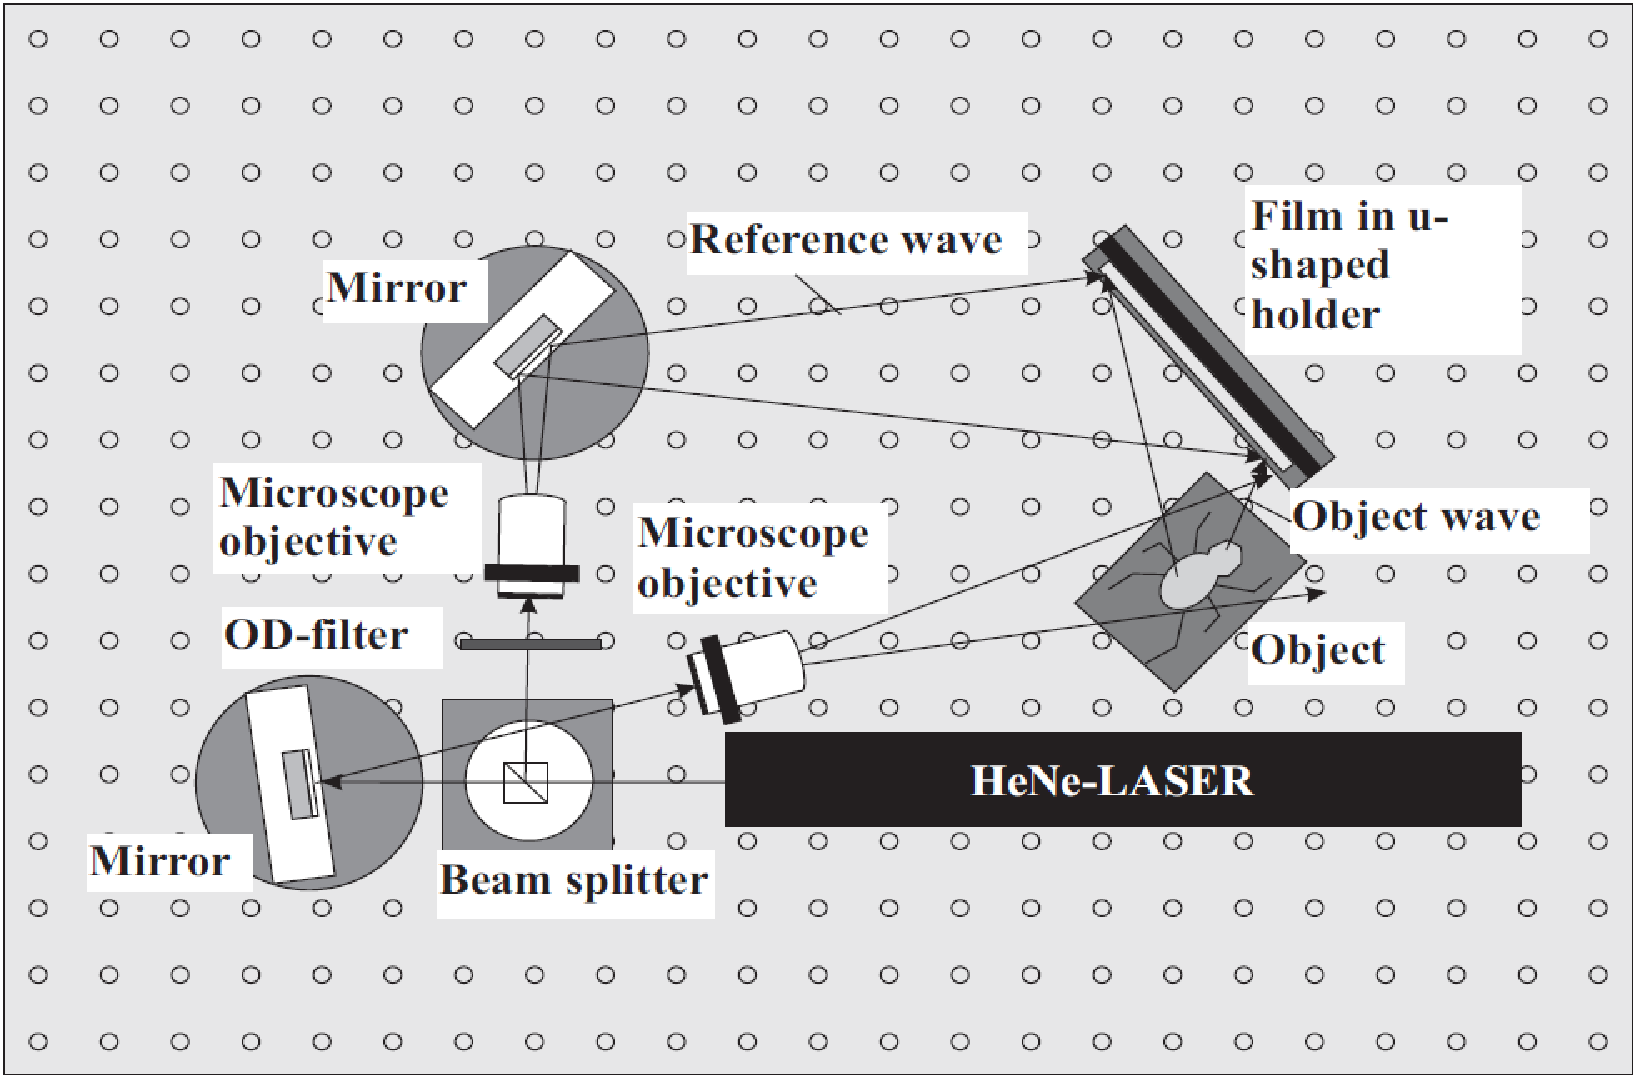
\includegraphics[width=0.5\textwidth]{graphics/aufbau_transmiss}
  \caption{Set-up for taking a transmission hologram}
  \label{fig:aufbau_transmiss}
\end{figure}
First of all one has to consider that the object and the holographic film are illuminated homogeneously. But due to reasons of coherence it is also important that the difference in pathlength of object and reference beam does not exceed approximately $\unit[30]{cm}$. Furthermore one inserts an OD filter into the reference beam to adjust the intensities of both beams. If everything is aligned properly the light is switched off except for a small LED panel and the exposure of the holographic film is done for $\unit[5]{s}$. Then the film is developed like explained in the description~\cite{skript}. For reconstruction of the object the film is placed at its position of recording, the object is removed and the object beam is blocked. Now we are indeed able to observe a three dimensional transmission hologram at the former position of the object (see figure \ref{fig:transmiss}). Unfortunately we missed to remove the OD filter while exposing the film. Therefore our hologram is weaker than it was supposed to be. Additionally the angle range for observation is rather small.
\begin{figure}[H]
    \begin{minipage}{0.2\textheight}
  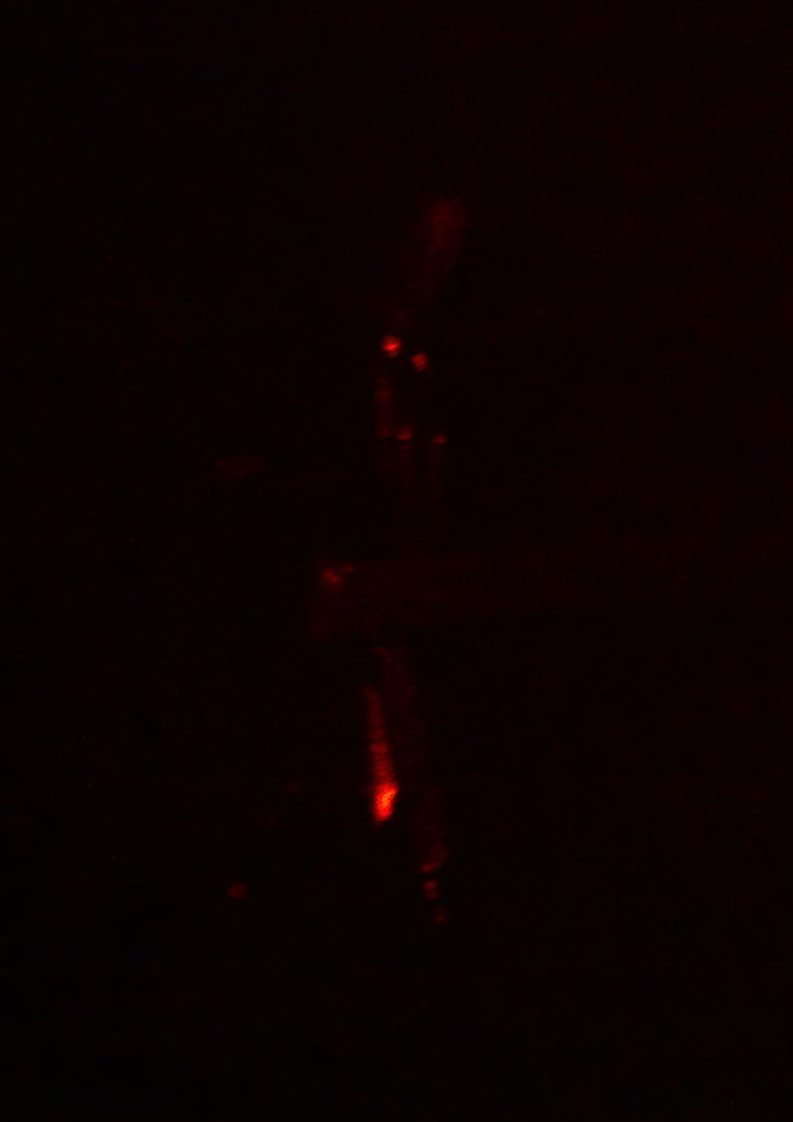
\includegraphics[width=1.0\textwidth]{graphics/transmiss1}
    \end{minipage}
    \hspace{1.3cm}
    \begin{minipage}{0.17\textheight}
  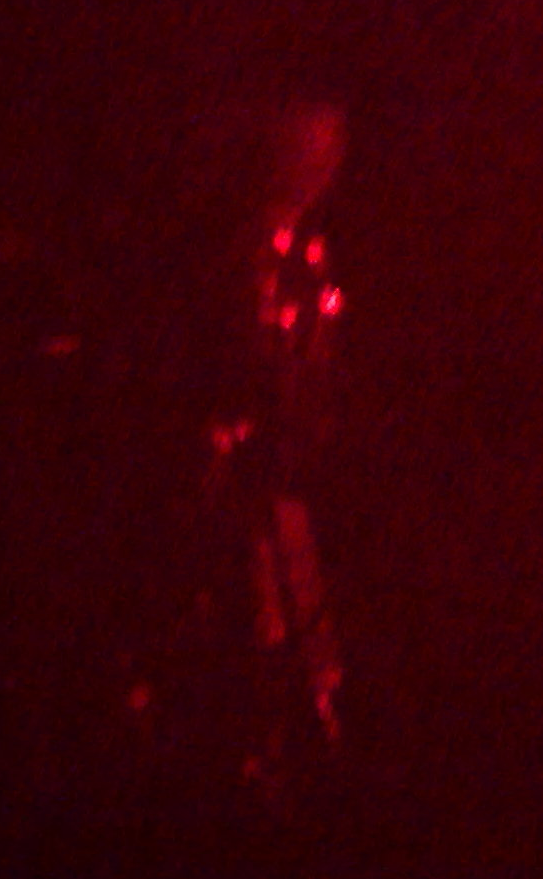
\includegraphics[width=1.0\textwidth]{graphics/transmiss2}
    \end{minipage}
  \caption{Photographs of our transmission hologram}
  \label{fig:transmiss}
\end{figure}
If one uses normal light only a spectral pattern due to the mentioned grating-like structure of the developed film is observed.

\subsubsection{Reflection Hologram}


\subsection{Holography with Lithium Niobate}
\label{subsec:ana_linbo3}
\subsubsection{Recording the Writing Curve}
\label{subsubsec:ana_writing}
In this part of the experiment we want to store a transmission phase hologram in a photorefractive lithium niobate crystal. In oder to do this we set up the experiment as shown in figure \ref{fig:setup_writing}.
\begin{figure}[H]
	\centering
		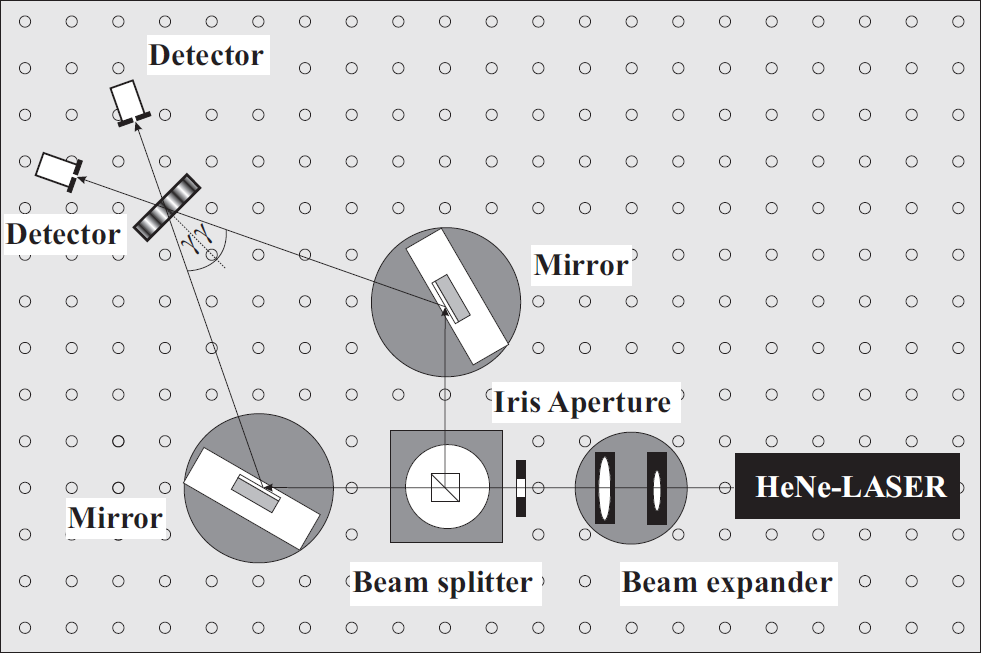
\includegraphics[width=0.5\textwidth]{graphics/setup_writing}
	\caption{Setup for recording the writing curve \cite{skript}}
	\label{fig:setup_writing}
\end{figure}
We adjust the angle between the normal to the recording surface and the writing beams to $\gamma = \unit[(20.0\pm 0.2)]{^\circ}$. Therefore the angle between the two beams inside the crystal is given by the \textsc{Snellius'} law:
\begin{align}
2\theta = 2\arcsin\left(\frac{n_\textrm{Air}}{n_\textrm{crystal}}\sin\gamma\right) = \unit[(8.6 \pm 0.4)]{^\circ}
\end{align}
because the refractive index of the \linbo crystal is given by $n_\textrm{crystal} = \unit[2.29]{}$ for light with a wavelength of $\lambda = \unit[633]{nm}$.
After having optimized the setup we illuminate the crystal with a tungsten lamp for around one hour to erase possibly existing holograms. 

Now we block the laser and perform background measurements for both photodiodes. Because they are connected to an amplifier, we do the measurement for each range. The results are displayed in table \ref{tab:ana_background}. Eventually we are ready to record the writing curve. We unblock the laser and measure the diffraction effiency in time intervalls of about one minute. To measure the intensities we block one of the writing beams so one of the photodiodes measures the diffracted and the other one the transmitted intensity.

\begin{table}[H]
  \centering
\resizebox{0.5\textwidth}{!}{
  \begin{tabular}{l|cc}
    \toprule
     Range & $I_\textrm{diff}^\textrm{bgd}$ [$\unit[]{mW}$] & $I_\textrm{trans}^\textrm{bgd}$ [$\unit[]{mW}$]\\
    \midrule[0.75pt]
$3$ & $-4.0 \pm 0.5$ & $0.0 \pm 0.5$\\
$4$ & $-4.0 \pm 0.5$ & $0.0 \pm 0.5$\\
$5$ & $-4.0 \pm 0.5$ & $0.0 \pm 0.5$\\
$6$ & $-4.0 \pm 0.5$ & $0.0 \pm 0.5$\\
$7$ & $-2.0 \pm 0.5$ & $2.0 \pm 0.5$\\
$8$ & $17.0 \pm 0.5$ & $25.0 \pm 0.5$\\
    \bottomrule
  \end{tabular}
}
\caption{Background measurements for the two photodiodes}
  \label{tab:ana_background}
\end{table}

The first curve we recorded this way behaved well for the first 20 minutes, but then began contrary to our expectation to fall again. Indeed a reflection went through the crystal again an therefore it was deleted right after beiing written. So we realigned our setup, dropped the data and restarted the measurement. The data is shown in tables \ref{tab:ana_writing_first} and \ref{tab:ana_writing_second} in the appendix and plotted in figure \ref{fig:ana_writing}.
\begin{figure}[H]
\begin{floatrow}
\resizebox{0.5\textwidth}{!}{
	\begin{tikzpicture}[gnuplot]
%% generated with GNUPLOT 4.4p0 (Lua 5.1.4; terminal rev. 97, script rev. 96a)
%% 09.05.2010 23:59:42
\gpcolor{gp lt color border}
\gpsetlinetype{gp lt border}
\gpsetlinewidth{1.00}
\draw[gp path] (1.504,0.985)--(1.684,0.985);
\draw[gp path] (12.039,0.985)--(11.859,0.985);
\node[gp node right] at (1.320,0.985) { 0};
\draw[gp path] (1.504,2.042)--(1.684,2.042);
\draw[gp path] (12.039,2.042)--(11.859,2.042);
\node[gp node right] at (1.320,2.042) { 2};
\draw[gp path] (1.504,3.098)--(1.684,3.098);
\draw[gp path] (12.039,3.098)--(11.859,3.098);
\node[gp node right] at (1.320,3.098) { 4};
\draw[gp path] (1.504,4.155)--(1.684,4.155);
\draw[gp path] (12.039,4.155)--(11.859,4.155);
\node[gp node right] at (1.320,4.155) { 6};
\draw[gp path] (1.504,5.211)--(1.684,5.211);
\draw[gp path] (12.039,5.211)--(11.859,5.211);
\node[gp node right] at (1.320,5.211) { 8};
\draw[gp path] (1.504,6.268)--(1.684,6.268);
\draw[gp path] (12.039,6.268)--(11.859,6.268);
\node[gp node right] at (1.320,6.268) { 10};
\draw[gp path] (1.504,7.324)--(1.684,7.324);
\draw[gp path] (12.039,7.324)--(11.859,7.324);
\node[gp node right] at (1.320,7.324) { 12};
\draw[gp path] (1.504,8.381)--(1.684,8.381);
\draw[gp path] (12.039,8.381)--(11.859,8.381);
\node[gp node right] at (1.320,8.381) { 14};
\draw[gp path] (1.504,0.985)--(1.504,1.165);
\draw[gp path] (1.504,8.381)--(1.504,8.201);
\node[gp node center] at (1.504,0.677) { 0};
\draw[gp path] (3.203,0.985)--(3.203,1.165);
\draw[gp path] (3.203,8.381)--(3.203,8.201);
\node[gp node center] at (3.203,0.677) { 500};
\draw[gp path] (4.902,0.985)--(4.902,1.165);
\draw[gp path] (4.902,8.381)--(4.902,8.201);
\node[gp node center] at (4.902,0.677) { 1000};
\draw[gp path] (6.602,0.985)--(6.602,1.165);
\draw[gp path] (6.602,8.381)--(6.602,8.201);
\node[gp node center] at (6.602,0.677) { 1500};
\draw[gp path] (8.301,0.985)--(8.301,1.165);
\draw[gp path] (8.301,8.381)--(8.301,8.201);
\node[gp node center] at (8.301,0.677) { 2000};
\draw[gp path] (10.000,0.985)--(10.000,1.165);
\draw[gp path] (10.000,8.381)--(10.000,8.201);
\node[gp node center] at (10.000,0.677) { 2500};
\draw[gp path] (11.699,0.985)--(11.699,1.165);
\draw[gp path] (11.699,8.381)--(11.699,8.201);
\node[gp node center] at (11.699,0.677) { 3000};
\draw[gp path] (1.504,8.381)--(1.504,0.985)--(12.039,0.985)--(12.039,8.381)--cycle;
\node[gp node center,rotate=-270] at (0.430,4.683) {$\eta$ [$\unit[]{10^{-3}}$]};
\node[gp node center] at (6.771,0.215) {t [s]};
\node[gp node right] at (10.571,8.047) {Measured Data};
\gpcolor{gp lt color 0}
\gpsetlinetype{gp lt plot 0}
\draw[gp path] (10.755,8.047)--(11.671,8.047);
\draw[gp path] (10.755,8.137)--(10.755,7.957);
\draw[gp path] (11.671,8.137)--(11.671,7.957);
\draw[gp path] (1.504,1.019)--(1.504,1.020);
\draw[gp path] (1.414,1.019)--(1.594,1.019);
\draw[gp path] (1.414,1.020)--(1.594,1.020);
\draw[gp path] (1.636,1.044)--(1.816,1.044);
\draw[gp path] (1.636,1.044)--(1.816,1.044);
\draw[gp path] (1.948,1.091)--(1.948,1.092);
\draw[gp path] (1.858,1.091)--(2.038,1.091);
\draw[gp path] (1.858,1.092)--(2.038,1.092);
\draw[gp path] (2.181,1.115)--(2.181,1.116);
\draw[gp path] (2.091,1.115)--(2.271,1.115);
\draw[gp path] (2.091,1.116)--(2.271,1.116);
\draw[gp path] (2.368,1.150)--(2.368,1.151);
\draw[gp path] (2.278,1.150)--(2.458,1.150);
\draw[gp path] (2.278,1.151)--(2.458,1.151);
\draw[gp path] (2.542,1.191)--(2.542,1.192);
\draw[gp path] (2.452,1.191)--(2.632,1.191);
\draw[gp path] (2.452,1.192)--(2.632,1.192);
\draw[gp path] (2.737,1.233)--(2.737,1.235);
\draw[gp path] (2.647,1.233)--(2.827,1.233);
\draw[gp path] (2.647,1.235)--(2.827,1.235);
\draw[gp path] (2.964,1.263)--(2.964,1.264);
\draw[gp path] (2.874,1.263)--(3.054,1.263);
\draw[gp path] (2.874,1.264)--(3.054,1.264);
\draw[gp path] (3.136,1.315)--(3.136,1.316);
\draw[gp path] (3.046,1.315)--(3.226,1.315);
\draw[gp path] (3.046,1.316)--(3.226,1.316);
\draw[gp path] (3.361,1.364)--(3.361,1.365);
\draw[gp path] (3.271,1.364)--(3.451,1.364);
\draw[gp path] (3.271,1.365)--(3.451,1.365);
\draw[gp path] (3.574,1.419)--(3.574,1.420);
\draw[gp path] (3.484,1.419)--(3.664,1.419);
\draw[gp path] (3.484,1.420)--(3.664,1.420);
\draw[gp path] (3.796,1.468)--(3.796,1.470);
\draw[gp path] (3.706,1.468)--(3.886,1.468);
\draw[gp path] (3.706,1.470)--(3.886,1.470);
\draw[gp path] (3.995,1.536)--(3.995,1.537);
\draw[gp path] (3.905,1.536)--(4.085,1.536);
\draw[gp path] (3.905,1.537)--(4.085,1.537);
\draw[gp path] (4.218,1.590)--(4.218,1.591);
\draw[gp path] (4.128,1.590)--(4.308,1.590);
\draw[gp path] (4.128,1.591)--(4.308,1.591);
\draw[gp path] (4.456,1.640)--(4.456,1.641);
\draw[gp path] (4.366,1.640)--(4.546,1.640);
\draw[gp path] (4.366,1.641)--(4.546,1.641);
\draw[gp path] (4.627,1.710)--(4.627,1.712);
\draw[gp path] (4.537,1.710)--(4.717,1.710);
\draw[gp path] (4.537,1.712)--(4.717,1.712);
\draw[gp path] (4.852,1.766)--(4.852,1.768);
\draw[gp path] (4.762,1.766)--(4.942,1.766);
\draw[gp path] (4.762,1.768)--(4.942,1.768);
\draw[gp path] (5.078,1.830)--(5.078,1.831);
\draw[gp path] (4.988,1.830)--(5.168,1.830);
\draw[gp path] (4.988,1.831)--(5.168,1.831);
\draw[gp path] (5.294,1.898)--(5.294,1.900);
\draw[gp path] (5.204,1.898)--(5.384,1.898);
\draw[gp path] (5.204,1.900)--(5.384,1.900);
\draw[gp path] (5.486,1.981)--(5.486,1.991);
\draw[gp path] (5.396,1.981)--(5.576,1.981);
\draw[gp path] (5.396,1.991)--(5.576,1.991);
\draw[gp path] (5.717,2.064)--(5.717,2.074);
\draw[gp path] (5.627,2.064)--(5.807,2.064);
\draw[gp path] (5.627,2.074)--(5.807,2.074);
\draw[gp path] (5.918,2.142)--(5.918,2.152);
\draw[gp path] (5.828,2.142)--(6.008,2.142);
\draw[gp path] (5.828,2.152)--(6.008,2.152);
\draw[gp path] (6.137,2.225)--(6.137,2.235);
\draw[gp path] (6.047,2.225)--(6.227,2.225);
\draw[gp path] (6.047,2.235)--(6.227,2.235);
\draw[gp path] (6.308,2.300)--(6.308,2.310);
\draw[gp path] (6.218,2.300)--(6.398,2.300);
\draw[gp path] (6.218,2.310)--(6.398,2.310);
\draw[gp path] (6.544,2.400)--(6.544,2.410);
\draw[gp path] (6.454,2.400)--(6.634,2.400);
\draw[gp path] (6.454,2.410)--(6.634,2.410);
\draw[gp path] (6.772,2.483)--(6.772,2.493);
\draw[gp path] (6.682,2.483)--(6.862,2.483);
\draw[gp path] (6.682,2.493)--(6.862,2.493);
\draw[gp path] (6.978,2.596)--(6.978,2.606);
\draw[gp path] (6.888,2.596)--(7.068,2.596);
\draw[gp path] (6.888,2.606)--(7.068,2.606);
\draw[gp path] (7.179,2.710)--(7.179,2.720);
\draw[gp path] (7.089,2.710)--(7.269,2.710);
\draw[gp path] (7.089,2.720)--(7.269,2.720);
\draw[gp path] (7.375,2.831)--(7.375,2.841);
\draw[gp path] (7.285,2.831)--(7.465,2.831);
\draw[gp path] (7.285,2.841)--(7.465,2.841);
\draw[gp path] (7.604,2.951)--(7.604,2.962);
\draw[gp path] (7.514,2.951)--(7.694,2.951);
\draw[gp path] (7.514,2.962)--(7.694,2.962);
\draw[gp path] (7.780,3.105)--(7.780,3.115);
\draw[gp path] (7.690,3.105)--(7.870,3.105);
\draw[gp path] (7.690,3.115)--(7.870,3.115);
\draw[gp path] (7.999,3.229)--(7.999,3.240);
\draw[gp path] (7.909,3.229)--(8.089,3.229);
\draw[gp path] (7.909,3.240)--(8.089,3.240);
\draw[gp path] (8.197,3.367)--(8.197,3.377);
\draw[gp path] (8.107,3.367)--(8.287,3.367);
\draw[gp path] (8.107,3.377)--(8.287,3.377);
\draw[gp path] (8.432,3.534)--(8.432,3.545);
\draw[gp path] (8.342,3.534)--(8.522,3.534);
\draw[gp path] (8.342,3.545)--(8.522,3.545);
\draw[gp path] (8.652,3.691)--(8.652,3.702);
\draw[gp path] (8.562,3.691)--(8.742,3.691);
\draw[gp path] (8.562,3.702)--(8.742,3.702);
\draw[gp path] (8.863,3.835)--(8.863,3.846);
\draw[gp path] (8.773,3.835)--(8.953,3.835);
\draw[gp path] (8.773,3.846)--(8.953,3.846);
\draw[gp path] (9.072,4.025)--(9.072,4.036);
\draw[gp path] (8.982,4.025)--(9.162,4.025);
\draw[gp path] (8.982,4.036)--(9.162,4.036);
\draw[gp path] (9.295,4.214)--(9.295,4.226);
\draw[gp path] (9.205,4.214)--(9.385,4.214);
\draw[gp path] (9.205,4.226)--(9.385,4.226);
\draw[gp path] (9.492,4.384)--(9.492,4.396);
\draw[gp path] (9.402,4.384)--(9.582,4.384);
\draw[gp path] (9.402,4.396)--(9.582,4.396);
\draw[gp path] (9.666,4.576)--(9.666,4.588);
\draw[gp path] (9.576,4.576)--(9.756,4.576);
\draw[gp path] (9.576,4.588)--(9.756,4.588);
\draw[gp path] (9.896,4.801)--(9.896,4.812);
\draw[gp path] (9.806,4.801)--(9.986,4.801);
\draw[gp path] (9.806,4.812)--(9.986,4.812);
\draw[gp path] (10.068,5.029)--(10.068,5.041);
\draw[gp path] (9.978,5.029)--(10.158,5.029);
\draw[gp path] (9.978,5.041)--(10.158,5.041);
\draw[gp path] (10.295,5.250)--(10.295,5.263);
\draw[gp path] (10.205,5.250)--(10.385,5.250);
\draw[gp path] (10.205,5.263)--(10.385,5.263);
\draw[gp path] (10.491,5.490)--(10.491,5.502);
\draw[gp path] (10.401,5.490)--(10.581,5.490);
\draw[gp path] (10.401,5.502)--(10.581,5.502);
\draw[gp path] (10.666,5.770)--(10.666,5.783);
\draw[gp path] (10.576,5.770)--(10.756,5.770);
\draw[gp path] (10.576,5.783)--(10.756,5.783);
\draw[gp path] (10.895,6.026)--(10.895,6.039);
\draw[gp path] (10.805,6.026)--(10.985,6.026);
\draw[gp path] (10.805,6.039)--(10.985,6.039);
\draw[gp path] (11.107,6.288)--(11.107,6.302);
\draw[gp path] (11.017,6.288)--(11.197,6.288);
\draw[gp path] (11.017,6.302)--(11.197,6.302);
\draw[gp path] (11.332,6.595)--(11.332,6.609);
\draw[gp path] (11.242,6.595)--(11.422,6.595);
\draw[gp path] (11.242,6.609)--(11.422,6.609);
\draw[gp path] (11.546,6.865)--(11.546,6.879);
\draw[gp path] (11.456,6.865)--(11.636,6.865);
\draw[gp path] (11.456,6.879)--(11.636,6.879);
\draw[gp path] (11.727,7.174)--(11.727,7.189);
\draw[gp path] (11.637,7.174)--(11.817,7.174);
\draw[gp path] (11.637,7.189)--(11.817,7.189);
\draw[gp path] (11.907,7.452)--(11.907,7.467);
\draw[gp path] (11.817,7.452)--(11.997,7.452);
\draw[gp path] (11.817,7.467)--(11.997,7.467);
\draw[gp path] (1.504,1.019)--(1.506,1.019);
\draw[gp path] (1.504,0.929)--(1.504,1.109);
\draw[gp path] (1.506,0.929)--(1.506,1.109);
\draw[gp path] (1.724,1.044)--(1.728,1.044);
\draw[gp path] (1.724,0.954)--(1.724,1.134);
\draw[gp path] (1.728,0.954)--(1.728,1.134);
\draw[gp path] (1.946,1.091)--(1.949,1.091);
\draw[gp path] (1.946,1.001)--(1.946,1.181);
\draw[gp path] (1.949,1.001)--(1.949,1.181);
\draw[gp path] (2.179,1.115)--(2.183,1.115);
\draw[gp path] (2.179,1.025)--(2.179,1.205);
\draw[gp path] (2.183,1.025)--(2.183,1.205);
\draw[gp path] (2.366,1.151)--(2.370,1.151);
\draw[gp path] (2.366,1.061)--(2.366,1.241);
\draw[gp path] (2.370,1.061)--(2.370,1.241);
\draw[gp path] (2.540,1.191)--(2.543,1.191);
\draw[gp path] (2.540,1.101)--(2.540,1.281);
\draw[gp path] (2.543,1.101)--(2.543,1.281);
\draw[gp path] (2.735,1.234)--(2.739,1.234);
\draw[gp path] (2.735,1.144)--(2.735,1.324);
\draw[gp path] (2.739,1.144)--(2.739,1.324);
\draw[gp path] (2.962,1.263)--(2.965,1.263);
\draw[gp path] (2.962,1.173)--(2.962,1.353);
\draw[gp path] (2.965,1.173)--(2.965,1.353);
\draw[gp path] (3.135,1.315)--(3.138,1.315);
\draw[gp path] (3.135,1.225)--(3.135,1.405);
\draw[gp path] (3.138,1.225)--(3.138,1.405);
\draw[gp path] (3.359,1.364)--(3.363,1.364);
\draw[gp path] (3.359,1.274)--(3.359,1.454);
\draw[gp path] (3.363,1.274)--(3.363,1.454);
\draw[gp path] (3.572,1.419)--(3.575,1.419);
\draw[gp path] (3.572,1.329)--(3.572,1.509);
\draw[gp path] (3.575,1.329)--(3.575,1.509);
\draw[gp path] (3.794,1.469)--(3.797,1.469);
\draw[gp path] (3.794,1.379)--(3.794,1.559);
\draw[gp path] (3.797,1.379)--(3.797,1.559);
\draw[gp path] (3.993,1.537)--(3.997,1.537);
\draw[gp path] (3.993,1.447)--(3.993,1.627);
\draw[gp path] (3.997,1.447)--(3.997,1.627);
\draw[gp path] (4.217,1.590)--(4.220,1.590);
\draw[gp path] (4.217,1.500)--(4.217,1.680);
\draw[gp path] (4.220,1.500)--(4.220,1.680);
\draw[gp path] (4.454,1.640)--(4.458,1.640);
\draw[gp path] (4.454,1.550)--(4.454,1.730);
\draw[gp path] (4.458,1.550)--(4.458,1.730);
\draw[gp path] (4.625,1.711)--(4.628,1.711);
\draw[gp path] (4.625,1.621)--(4.625,1.801);
\draw[gp path] (4.628,1.621)--(4.628,1.801);
\draw[gp path] (4.850,1.767)--(4.854,1.767);
\draw[gp path] (4.850,1.677)--(4.850,1.857);
\draw[gp path] (4.854,1.677)--(4.854,1.857);
\draw[gp path] (5.077,1.831)--(5.080,1.831);
\draw[gp path] (5.077,1.741)--(5.077,1.921);
\draw[gp path] (5.080,1.741)--(5.080,1.921);
\draw[gp path] (5.292,1.899)--(5.295,1.899);
\draw[gp path] (5.292,1.809)--(5.292,1.989);
\draw[gp path] (5.295,1.809)--(5.295,1.989);
\draw[gp path] (5.484,1.986)--(5.488,1.986);
\draw[gp path] (5.484,1.896)--(5.484,2.076);
\draw[gp path] (5.488,1.896)--(5.488,2.076);
\draw[gp path] (5.715,2.069)--(5.718,2.069);
\draw[gp path] (5.715,1.979)--(5.715,2.159);
\draw[gp path] (5.718,1.979)--(5.718,2.159);
\draw[gp path] (5.916,2.147)--(5.920,2.147);
\draw[gp path] (5.916,2.057)--(5.916,2.237);
\draw[gp path] (5.920,2.057)--(5.920,2.237);
\draw[gp path] (6.135,2.230)--(6.138,2.230);
\draw[gp path] (6.135,2.140)--(6.135,2.320);
\draw[gp path] (6.138,2.140)--(6.138,2.320);
\draw[gp path] (6.306,2.305)--(6.310,2.305);
\draw[gp path] (6.306,2.215)--(6.306,2.395);
\draw[gp path] (6.310,2.215)--(6.310,2.395);
\draw[gp path] (6.543,2.405)--(6.546,2.405);
\draw[gp path] (6.543,2.315)--(6.543,2.495);
\draw[gp path] (6.546,2.315)--(6.546,2.495);
\draw[gp path] (6.770,2.488)--(6.774,2.488);
\draw[gp path] (6.770,2.398)--(6.770,2.578);
\draw[gp path] (6.774,2.398)--(6.774,2.578);
\draw[gp path] (6.976,2.601)--(6.980,2.601);
\draw[gp path] (6.976,2.511)--(6.976,2.691);
\draw[gp path] (6.980,2.511)--(6.980,2.691);
\draw[gp path] (7.177,2.715)--(7.181,2.715);
\draw[gp path] (7.177,2.625)--(7.177,2.805);
\draw[gp path] (7.181,2.625)--(7.181,2.805);
\draw[gp path] (7.373,2.836)--(7.376,2.836);
\draw[gp path] (7.373,2.746)--(7.373,2.926);
\draw[gp path] (7.376,2.746)--(7.376,2.926);
\draw[gp path] (7.603,2.956)--(7.606,2.956);
\draw[gp path] (7.603,2.866)--(7.603,3.046);
\draw[gp path] (7.606,2.866)--(7.606,3.046);
\draw[gp path] (7.778,3.110)--(7.782,3.110);
\draw[gp path] (7.778,3.020)--(7.778,3.200);
\draw[gp path] (7.782,3.020)--(7.782,3.200);
\draw[gp path] (7.998,3.235)--(8.001,3.235);
\draw[gp path] (7.998,3.145)--(7.998,3.325);
\draw[gp path] (8.001,3.145)--(8.001,3.325);
\draw[gp path] (8.195,3.372)--(8.199,3.372);
\draw[gp path] (8.195,3.282)--(8.195,3.462);
\draw[gp path] (8.199,3.282)--(8.199,3.462);
\draw[gp path] (8.430,3.539)--(8.434,3.539);
\draw[gp path] (8.430,3.449)--(8.430,3.629);
\draw[gp path] (8.434,3.449)--(8.434,3.629);
\draw[gp path] (8.650,3.697)--(8.654,3.697);
\draw[gp path] (8.650,3.607)--(8.650,3.787);
\draw[gp path] (8.654,3.607)--(8.654,3.787);
\draw[gp path] (8.861,3.841)--(8.865,3.841);
\draw[gp path] (8.861,3.751)--(8.861,3.931);
\draw[gp path] (8.865,3.751)--(8.865,3.931);
\draw[gp path] (9.070,4.031)--(9.073,4.031);
\draw[gp path] (9.070,3.941)--(9.070,4.121);
\draw[gp path] (9.073,3.941)--(9.073,4.121);
\draw[gp path] (9.293,4.220)--(9.296,4.220);
\draw[gp path] (9.293,4.130)--(9.293,4.310);
\draw[gp path] (9.296,4.130)--(9.296,4.310);
\draw[gp path] (9.490,4.390)--(9.494,4.390);
\draw[gp path] (9.490,4.300)--(9.490,4.480);
\draw[gp path] (9.494,4.300)--(9.494,4.480);
\draw[gp path] (9.664,4.582)--(9.668,4.582);
\draw[gp path] (9.664,4.492)--(9.664,4.672);
\draw[gp path] (9.668,4.492)--(9.668,4.672);
\draw[gp path] (9.894,4.806)--(9.898,4.806);
\draw[gp path] (9.894,4.716)--(9.894,4.896);
\draw[gp path] (9.898,4.716)--(9.898,4.896);
\draw[gp path] (10.067,5.035)--(10.070,5.035);
\draw[gp path] (10.067,4.945)--(10.067,5.125);
\draw[gp path] (10.070,4.945)--(10.070,5.125);
\draw[gp path] (10.293,5.257)--(10.297,5.257);
\draw[gp path] (10.293,5.167)--(10.293,5.347);
\draw[gp path] (10.297,5.167)--(10.297,5.347);
\draw[gp path] (10.489,5.496)--(10.493,5.496);
\draw[gp path] (10.489,5.406)--(10.489,5.586);
\draw[gp path] (10.493,5.406)--(10.493,5.586);
\draw[gp path] (10.664,5.776)--(10.668,5.776);
\draw[gp path] (10.664,5.686)--(10.664,5.866);
\draw[gp path] (10.668,5.686)--(10.668,5.866);
\draw[gp path] (10.894,6.032)--(10.897,6.032);
\draw[gp path] (10.894,5.942)--(10.894,6.122);
\draw[gp path] (10.897,5.942)--(10.897,6.122);
\draw[gp path] (11.105,6.295)--(11.109,6.295);
\draw[gp path] (11.105,6.205)--(11.105,6.385);
\draw[gp path] (11.109,6.205)--(11.109,6.385);
\draw[gp path] (11.331,6.602)--(11.334,6.602);
\draw[gp path] (11.331,6.512)--(11.331,6.692);
\draw[gp path] (11.334,6.512)--(11.334,6.692);
\draw[gp path] (11.544,6.872)--(11.547,6.872);
\draw[gp path] (11.544,6.782)--(11.544,6.962);
\draw[gp path] (11.547,6.782)--(11.547,6.962);
\draw[gp path] (11.725,7.181)--(11.728,7.181);
\draw[gp path] (11.725,7.091)--(11.725,7.271);
\draw[gp path] (11.728,7.091)--(11.728,7.271);
\draw[gp path] (11.905,7.459)--(11.909,7.459);
\draw[gp path] (11.905,7.369)--(11.905,7.549);
\draw[gp path] (11.909,7.369)--(11.909,7.549);
\gpsetpointsize{4.00}
\gppoint{gp mark 1}{(1.504,1.019)}
\gppoint{gp mark 1}{(1.726,1.044)}
\gppoint{gp mark 1}{(1.948,1.091)}
\gppoint{gp mark 1}{(2.181,1.115)}
\gppoint{gp mark 1}{(2.368,1.151)}
\gppoint{gp mark 1}{(2.542,1.191)}
\gppoint{gp mark 1}{(2.737,1.234)}
\gppoint{gp mark 1}{(2.964,1.263)}
\gppoint{gp mark 1}{(3.136,1.315)}
\gppoint{gp mark 1}{(3.361,1.364)}
\gppoint{gp mark 1}{(3.574,1.419)}
\gppoint{gp mark 1}{(3.796,1.469)}
\gppoint{gp mark 1}{(3.995,1.537)}
\gppoint{gp mark 1}{(4.218,1.590)}
\gppoint{gp mark 1}{(4.456,1.640)}
\gppoint{gp mark 1}{(4.627,1.711)}
\gppoint{gp mark 1}{(4.852,1.767)}
\gppoint{gp mark 1}{(5.078,1.831)}
\gppoint{gp mark 1}{(5.294,1.899)}
\gppoint{gp mark 1}{(5.486,1.986)}
\gppoint{gp mark 1}{(5.717,2.069)}
\gppoint{gp mark 1}{(5.918,2.147)}
\gppoint{gp mark 1}{(6.137,2.230)}
\gppoint{gp mark 1}{(6.308,2.305)}
\gppoint{gp mark 1}{(6.544,2.405)}
\gppoint{gp mark 1}{(6.772,2.488)}
\gppoint{gp mark 1}{(6.978,2.601)}
\gppoint{gp mark 1}{(7.179,2.715)}
\gppoint{gp mark 1}{(7.375,2.836)}
\gppoint{gp mark 1}{(7.604,2.956)}
\gppoint{gp mark 1}{(7.780,3.110)}
\gppoint{gp mark 1}{(7.999,3.235)}
\gppoint{gp mark 1}{(8.197,3.372)}
\gppoint{gp mark 1}{(8.432,3.539)}
\gppoint{gp mark 1}{(8.652,3.697)}
\gppoint{gp mark 1}{(8.863,3.841)}
\gppoint{gp mark 1}{(9.072,4.031)}
\gppoint{gp mark 1}{(9.295,4.220)}
\gppoint{gp mark 1}{(9.492,4.390)}
\gppoint{gp mark 1}{(9.666,4.582)}
\gppoint{gp mark 1}{(9.896,4.806)}
\gppoint{gp mark 1}{(10.068,5.035)}
\gppoint{gp mark 1}{(10.295,5.257)}
\gppoint{gp mark 1}{(10.491,5.496)}
\gppoint{gp mark 1}{(10.666,5.776)}
\gppoint{gp mark 1}{(10.895,6.032)}
\gppoint{gp mark 1}{(11.107,6.295)}
\gppoint{gp mark 1}{(11.332,6.602)}
\gppoint{gp mark 1}{(11.546,6.872)}
\gppoint{gp mark 1}{(11.727,7.181)}
\gppoint{gp mark 1}{(11.907,7.459)}
\gppoint{gp mark 1}{(11.213,8.047)}
\gpcolor{gp lt color border}
\gpsetlinetype{gp lt border}
\draw[gp path] (1.504,8.381)--(1.504,0.985)--(12.039,0.985)--(12.039,8.381)--cycle;
%% coordinates of the plot area
\gpdefrectangularnode{gp plot 1}{\pgfpoint{1.504cm}{0.985cm}}{\pgfpoint{12.039cm}{8.381cm}}
\end{tikzpicture}
%% gnuplot variables

}
\resizebox{0.5\textwidth}{!}{
	\begin{tikzpicture}[gnuplot]
%% generated with GNUPLOT 4.4p0 (Lua 5.1.4; terminal rev. 97, script rev. 96a)
%% 09.05.2010 23:59:42
\gpcolor{gp lt color border}
\gpsetlinetype{gp lt border}
\gpsetlinewidth{1.00}
\draw[gp path] (1.688,0.985)--(1.868,0.985);
\draw[gp path] (12.039,0.985)--(11.859,0.985);
\node[gp node right] at (1.504,0.985) { 0};
\draw[gp path] (1.688,2.218)--(1.868,2.218);
\draw[gp path] (12.039,2.218)--(11.859,2.218);
\node[gp node right] at (1.504,2.218) { 20};
\draw[gp path] (1.688,3.450)--(1.868,3.450);
\draw[gp path] (12.039,3.450)--(11.859,3.450);
\node[gp node right] at (1.504,3.450) { 40};
\draw[gp path] (1.688,4.683)--(1.868,4.683);
\draw[gp path] (12.039,4.683)--(11.859,4.683);
\node[gp node right] at (1.504,4.683) { 60};
\draw[gp path] (1.688,5.916)--(1.868,5.916);
\draw[gp path] (12.039,5.916)--(11.859,5.916);
\node[gp node right] at (1.504,5.916) { 80};
\draw[gp path] (1.688,7.148)--(1.868,7.148);
\draw[gp path] (12.039,7.148)--(11.859,7.148);
\node[gp node right] at (1.504,7.148) { 100};
\draw[gp path] (1.688,8.381)--(1.868,8.381);
\draw[gp path] (12.039,8.381)--(11.859,8.381);
\node[gp node right] at (1.504,8.381) { 120};
\draw[gp path] (1.688,0.985)--(1.688,1.165);
\draw[gp path] (1.688,8.381)--(1.688,8.201);
\node[gp node center] at (1.688,0.677) { 0};
\draw[gp path] (3.358,0.985)--(3.358,1.165);
\draw[gp path] (3.358,8.381)--(3.358,8.201);
\node[gp node center] at (3.358,0.677) { 500};
\draw[gp path] (5.027,0.985)--(5.027,1.165);
\draw[gp path] (5.027,8.381)--(5.027,8.201);
\node[gp node center] at (5.027,0.677) { 1000};
\draw[gp path] (6.697,0.985)--(6.697,1.165);
\draw[gp path] (6.697,8.381)--(6.697,8.201);
\node[gp node center] at (6.697,0.677) { 1500};
\draw[gp path] (8.366,0.985)--(8.366,1.165);
\draw[gp path] (8.366,8.381)--(8.366,8.201);
\node[gp node center] at (8.366,0.677) { 2000};
\draw[gp path] (10.036,0.985)--(10.036,1.165);
\draw[gp path] (10.036,8.381)--(10.036,8.201);
\node[gp node center] at (10.036,0.677) { 2500};
\draw[gp path] (11.705,0.985)--(11.705,1.165);
\draw[gp path] (11.705,8.381)--(11.705,8.201);
\node[gp node center] at (11.705,0.677) { 3000};
\draw[gp path] (1.688,8.381)--(1.688,0.985)--(12.039,0.985)--(12.039,8.381)--cycle;
\node[gp node center,rotate=-270] at (0.430,4.683) {$\Delta n$ [$\unit[]{10^{-7}}$]};
\node[gp node center] at (6.863,0.215) {t [s]};
\node[gp node right] at (10.571,8.047) {Measured Data};
\gpcolor{gp lt color 0}
\gpsetlinetype{gp lt plot 0}
\draw[gp path] (10.755,8.047)--(11.671,8.047);
\draw[gp path] (10.755,8.137)--(10.755,7.957);
\draw[gp path] (11.671,8.137)--(11.671,7.957);
\draw[gp path] (1.688,1.480)--(1.688,1.481);
\draw[gp path] (1.598,1.480)--(1.778,1.480);
\draw[gp path] (1.598,1.481)--(1.778,1.481);
\draw[gp path] (1.906,1.633)--(1.906,1.634);
\draw[gp path] (1.816,1.633)--(1.996,1.633);
\draw[gp path] (1.816,1.634)--(1.996,1.634);
\draw[gp path] (2.124,1.855)--(2.124,1.859);
\draw[gp path] (2.034,1.855)--(2.214,1.855);
\draw[gp path] (2.034,1.859)--(2.214,1.859);
\draw[gp path] (2.353,1.946)--(2.353,1.950);
\draw[gp path] (2.263,1.946)--(2.443,1.946);
\draw[gp path] (2.263,1.950)--(2.443,1.950);
\draw[gp path] (2.537,2.071)--(2.537,2.074);
\draw[gp path] (2.447,2.071)--(2.627,2.071);
\draw[gp path] (2.447,2.074)--(2.627,2.074);
\draw[gp path] (2.708,2.196)--(2.708,2.199);
\draw[gp path] (2.618,2.196)--(2.798,2.196);
\draw[gp path] (2.618,2.199)--(2.798,2.199);
\draw[gp path] (2.899,2.317)--(2.899,2.319);
\draw[gp path] (2.809,2.317)--(2.989,2.317);
\draw[gp path] (2.809,2.319)--(2.989,2.319);
\draw[gp path] (3.122,2.393)--(3.122,2.396);
\draw[gp path] (3.032,2.393)--(3.212,2.393);
\draw[gp path] (3.032,2.396)--(3.212,2.396);
\draw[gp path] (3.292,2.519)--(3.292,2.522);
\draw[gp path] (3.202,2.519)--(3.382,2.519);
\draw[gp path] (3.202,2.522)--(3.382,2.522);
\draw[gp path] (3.513,2.629)--(3.513,2.632);
\draw[gp path] (3.423,2.629)--(3.603,2.629);
\draw[gp path] (3.423,2.632)--(3.603,2.632);
\draw[gp path] (3.721,2.745)--(3.721,2.747);
\draw[gp path] (3.631,2.745)--(3.811,2.745);
\draw[gp path] (3.631,2.747)--(3.811,2.747);
\draw[gp path] (3.940,2.842)--(3.940,2.845);
\draw[gp path] (3.850,2.842)--(4.030,2.842);
\draw[gp path] (3.850,2.845)--(4.030,2.845);
\draw[gp path] (4.135,2.968)--(4.135,2.970);
\draw[gp path] (4.045,2.968)--(4.225,2.968);
\draw[gp path] (4.045,2.970)--(4.225,2.970);
\draw[gp path] (4.355,3.063)--(4.355,3.065);
\draw[gp path] (4.265,3.063)--(4.445,3.063);
\draw[gp path] (4.265,3.065)--(4.445,3.065);
\draw[gp path] (4.588,3.147)--(4.588,3.149);
\draw[gp path] (4.498,3.147)--(4.678,3.147);
\draw[gp path] (4.498,3.149)--(4.678,3.149);
\draw[gp path] (4.756,3.260)--(4.756,3.262);
\draw[gp path] (4.666,3.260)--(4.846,3.260);
\draw[gp path] (4.666,3.262)--(4.846,3.262);
\draw[gp path] (4.978,3.346)--(4.978,3.349);
\draw[gp path] (4.888,3.346)--(5.068,3.346);
\draw[gp path] (4.888,3.349)--(5.068,3.349);
\draw[gp path] (5.200,3.440)--(5.200,3.443);
\draw[gp path] (5.110,3.440)--(5.290,3.440);
\draw[gp path] (5.110,3.443)--(5.290,3.443);
\draw[gp path] (5.412,3.538)--(5.412,3.541);
\draw[gp path] (5.322,3.538)--(5.502,3.538);
\draw[gp path] (5.322,3.541)--(5.502,3.541);
\draw[gp path] (5.601,3.651)--(5.601,3.665);
\draw[gp path] (5.511,3.651)--(5.691,3.651);
\draw[gp path] (5.511,3.665)--(5.691,3.665);
\draw[gp path] (5.827,3.761)--(5.827,3.773);
\draw[gp path] (5.737,3.761)--(5.917,3.761);
\draw[gp path] (5.737,3.773)--(5.917,3.773);
\draw[gp path] (6.025,3.859)--(6.025,3.871);
\draw[gp path] (5.935,3.859)--(6.115,3.859);
\draw[gp path] (5.935,3.871)--(6.115,3.871);
\draw[gp path] (6.240,3.960)--(6.240,3.972);
\draw[gp path] (6.150,3.960)--(6.330,3.960);
\draw[gp path] (6.150,3.972)--(6.330,3.972);
\draw[gp path] (6.408,4.049)--(6.408,4.060);
\draw[gp path] (6.318,4.049)--(6.498,4.049);
\draw[gp path] (6.318,4.060)--(6.498,4.060);
\draw[gp path] (6.640,4.164)--(6.640,4.175);
\draw[gp path] (6.550,4.164)--(6.730,4.164);
\draw[gp path] (6.550,4.175)--(6.730,4.175);
\draw[gp path] (6.864,4.255)--(6.864,4.266);
\draw[gp path] (6.774,4.255)--(6.954,4.255);
\draw[gp path] (6.774,4.266)--(6.954,4.266);
\draw[gp path] (7.066,4.377)--(7.066,4.388);
\draw[gp path] (6.976,4.377)--(7.156,4.377);
\draw[gp path] (6.976,4.388)--(7.156,4.388);
\draw[gp path] (7.264,4.495)--(7.264,4.506);
\draw[gp path] (7.174,4.495)--(7.354,4.495);
\draw[gp path] (7.174,4.506)--(7.354,4.506);
\draw[gp path] (7.456,4.616)--(7.456,4.626);
\draw[gp path] (7.366,4.616)--(7.546,4.616);
\draw[gp path] (7.366,4.626)--(7.546,4.626);
\draw[gp path] (7.682,4.733)--(7.682,4.743);
\draw[gp path] (7.592,4.733)--(7.772,4.733);
\draw[gp path] (7.592,4.743)--(7.772,4.743);
\draw[gp path] (7.854,4.877)--(7.854,4.886);
\draw[gp path] (7.764,4.877)--(7.944,4.877);
\draw[gp path] (7.764,4.886)--(7.944,4.886);
\draw[gp path] (8.070,4.989)--(8.070,4.999);
\draw[gp path] (7.980,4.989)--(8.160,4.989);
\draw[gp path] (7.980,4.999)--(8.160,4.999);
\draw[gp path] (8.264,5.110)--(8.264,5.119);
\draw[gp path] (8.174,5.110)--(8.354,5.110);
\draw[gp path] (8.174,5.119)--(8.354,5.119);
\draw[gp path] (8.495,5.253)--(8.495,5.262);
\draw[gp path] (8.405,5.253)--(8.585,5.253);
\draw[gp path] (8.405,5.262)--(8.585,5.262);
\draw[gp path] (8.711,5.383)--(8.711,5.392);
\draw[gp path] (8.621,5.383)--(8.801,5.383);
\draw[gp path] (8.621,5.392)--(8.801,5.392);
\draw[gp path] (8.919,5.499)--(8.919,5.507);
\draw[gp path] (8.829,5.499)--(9.009,5.499);
\draw[gp path] (8.829,5.507)--(9.009,5.507);
\draw[gp path] (9.124,5.647)--(9.124,5.655);
\draw[gp path] (9.034,5.647)--(9.214,5.647);
\draw[gp path] (9.034,5.655)--(9.214,5.655);
\draw[gp path] (9.343,5.790)--(9.343,5.798);
\draw[gp path] (9.253,5.790)--(9.433,5.790);
\draw[gp path] (9.253,5.798)--(9.433,5.798);
\draw[gp path] (9.536,5.915)--(9.536,5.923);
\draw[gp path] (9.446,5.915)--(9.626,5.915);
\draw[gp path] (9.446,5.923)--(9.626,5.923);
\draw[gp path] (9.707,6.053)--(9.707,6.061);
\draw[gp path] (9.617,6.053)--(9.797,6.053);
\draw[gp path] (9.617,6.061)--(9.797,6.061);
\draw[gp path] (9.934,6.209)--(9.934,6.217);
\draw[gp path] (9.844,6.209)--(10.024,6.209);
\draw[gp path] (9.844,6.217)--(10.024,6.217);
\draw[gp path] (10.103,6.364)--(10.103,6.372);
\draw[gp path] (10.013,6.364)--(10.193,6.364);
\draw[gp path] (10.013,6.372)--(10.193,6.372);
\draw[gp path] (10.326,6.509)--(10.326,6.517);
\draw[gp path] (10.236,6.509)--(10.416,6.509);
\draw[gp path] (10.236,6.517)--(10.416,6.517);
\draw[gp path] (10.518,6.662)--(10.518,6.670);
\draw[gp path] (10.428,6.662)--(10.608,6.662);
\draw[gp path] (10.428,6.670)--(10.608,6.670);
\draw[gp path] (10.690,6.837)--(10.690,6.845);
\draw[gp path] (10.600,6.837)--(10.780,6.837);
\draw[gp path] (10.600,6.845)--(10.780,6.845);
\draw[gp path] (10.915,6.992)--(10.915,7.000);
\draw[gp path] (10.825,6.992)--(11.005,6.992);
\draw[gp path] (10.825,7.000)--(11.005,7.000);
\draw[gp path] (11.123,7.146)--(11.123,7.154);
\draw[gp path] (11.033,7.146)--(11.213,7.146);
\draw[gp path] (11.033,7.154)--(11.213,7.154);
\draw[gp path] (11.345,7.323)--(11.345,7.331);
\draw[gp path] (11.255,7.323)--(11.435,7.323);
\draw[gp path] (11.255,7.331)--(11.435,7.331);
\draw[gp path] (11.554,7.474)--(11.554,7.482);
\draw[gp path] (11.464,7.474)--(11.644,7.474);
\draw[gp path] (11.464,7.482)--(11.644,7.482);
\draw[gp path] (11.732,7.643)--(11.732,7.651);
\draw[gp path] (11.642,7.643)--(11.822,7.643);
\draw[gp path] (11.642,7.651)--(11.822,7.651);
\draw[gp path] (11.909,7.792)--(11.909,7.800);
\draw[gp path] (11.819,7.792)--(11.999,7.792);
\draw[gp path] (11.819,7.800)--(11.999,7.800);
\draw[gp path] (1.688,1.481)--(1.690,1.481);
\draw[gp path] (1.688,1.391)--(1.688,1.571);
\draw[gp path] (1.690,1.391)--(1.690,1.571);
\draw[gp path] (1.904,1.633)--(1.908,1.633);
\draw[gp path] (1.904,1.543)--(1.904,1.723);
\draw[gp path] (1.908,1.543)--(1.908,1.723);
\draw[gp path] (2.122,1.857)--(2.126,1.857);
\draw[gp path] (2.122,1.767)--(2.122,1.947);
\draw[gp path] (2.126,1.767)--(2.126,1.947);
\draw[gp path] (2.352,1.948)--(2.355,1.948);
\draw[gp path] (2.352,1.858)--(2.352,2.038);
\draw[gp path] (2.355,1.858)--(2.355,2.038);
\draw[gp path] (2.535,2.073)--(2.538,2.073);
\draw[gp path] (2.535,1.983)--(2.535,2.163);
\draw[gp path] (2.538,1.983)--(2.538,2.163);
\draw[gp path] (2.706,2.198)--(2.709,2.198);
\draw[gp path] (2.706,2.108)--(2.706,2.288);
\draw[gp path] (2.709,2.108)--(2.709,2.288);
\draw[gp path] (2.898,2.318)--(2.901,2.318);
\draw[gp path] (2.898,2.228)--(2.898,2.408);
\draw[gp path] (2.901,2.228)--(2.901,2.408);
\draw[gp path] (3.121,2.394)--(3.124,2.394);
\draw[gp path] (3.121,2.304)--(3.121,2.484);
\draw[gp path] (3.124,2.304)--(3.124,2.484);
\draw[gp path] (3.290,2.520)--(3.293,2.520);
\draw[gp path] (3.290,2.430)--(3.290,2.610);
\draw[gp path] (3.293,2.430)--(3.293,2.610);
\draw[gp path] (3.511,2.630)--(3.514,2.630);
\draw[gp path] (3.511,2.540)--(3.511,2.720);
\draw[gp path] (3.514,2.540)--(3.514,2.720);
\draw[gp path] (3.720,2.746)--(3.723,2.746);
\draw[gp path] (3.720,2.656)--(3.720,2.836);
\draw[gp path] (3.723,2.656)--(3.723,2.836);
\draw[gp path] (3.938,2.843)--(3.941,2.843);
\draw[gp path] (3.938,2.753)--(3.938,2.933);
\draw[gp path] (3.941,2.753)--(3.941,2.933);
\draw[gp path] (4.134,2.969)--(4.137,2.969);
\draw[gp path] (4.134,2.879)--(4.134,3.059);
\draw[gp path] (4.137,2.879)--(4.137,3.059);
\draw[gp path] (4.353,3.064)--(4.357,3.064);
\draw[gp path] (4.353,2.974)--(4.353,3.154);
\draw[gp path] (4.357,2.974)--(4.357,3.154);
\draw[gp path] (4.587,3.148)--(4.590,3.148);
\draw[gp path] (4.587,3.058)--(4.587,3.238);
\draw[gp path] (4.590,3.058)--(4.590,3.238);
\draw[gp path] (4.754,3.261)--(4.758,3.261);
\draw[gp path] (4.754,3.171)--(4.754,3.351);
\draw[gp path] (4.758,3.171)--(4.758,3.351);
\draw[gp path] (4.976,3.348)--(4.979,3.348);
\draw[gp path] (4.976,3.258)--(4.976,3.438);
\draw[gp path] (4.979,3.258)--(4.979,3.438);
\draw[gp path] (5.198,3.442)--(5.202,3.442);
\draw[gp path] (5.198,3.352)--(5.198,3.532);
\draw[gp path] (5.202,3.352)--(5.202,3.532);
\draw[gp path] (5.410,3.539)--(5.413,3.539);
\draw[gp path] (5.410,3.449)--(5.410,3.629);
\draw[gp path] (5.413,3.449)--(5.413,3.629);
\draw[gp path] (5.599,3.658)--(5.602,3.658);
\draw[gp path] (5.599,3.568)--(5.599,3.748);
\draw[gp path] (5.602,3.568)--(5.602,3.748);
\draw[gp path] (5.825,3.767)--(5.829,3.767);
\draw[gp path] (5.825,3.677)--(5.825,3.857);
\draw[gp path] (5.829,3.677)--(5.829,3.857);
\draw[gp path] (6.023,3.865)--(6.027,3.865);
\draw[gp path] (6.023,3.775)--(6.023,3.955);
\draw[gp path] (6.027,3.775)--(6.027,3.955);
\draw[gp path] (6.238,3.966)--(6.241,3.966);
\draw[gp path] (6.238,3.876)--(6.238,4.056);
\draw[gp path] (6.241,3.876)--(6.241,4.056);
\draw[gp path] (6.406,4.055)--(6.410,4.055);
\draw[gp path] (6.406,3.965)--(6.406,4.145);
\draw[gp path] (6.410,3.965)--(6.410,4.145);
\draw[gp path] (6.639,4.170)--(6.642,4.170);
\draw[gp path] (6.639,4.080)--(6.639,4.260);
\draw[gp path] (6.642,4.080)--(6.642,4.260);
\draw[gp path] (6.862,4.261)--(6.866,4.261);
\draw[gp path] (6.862,4.171)--(6.862,4.351);
\draw[gp path] (6.866,4.171)--(6.866,4.351);
\draw[gp path] (7.065,4.383)--(7.068,4.383);
\draw[gp path] (7.065,4.293)--(7.065,4.473);
\draw[gp path] (7.068,4.293)--(7.068,4.473);
\draw[gp path] (7.262,4.500)--(7.266,4.500);
\draw[gp path] (7.262,4.410)--(7.262,4.590);
\draw[gp path] (7.266,4.410)--(7.266,4.590);
\draw[gp path] (7.454,4.621)--(7.458,4.621);
\draw[gp path] (7.454,4.531)--(7.454,4.711);
\draw[gp path] (7.458,4.531)--(7.458,4.711);
\draw[gp path] (7.680,4.738)--(7.683,4.738);
\draw[gp path] (7.680,4.648)--(7.680,4.828);
\draw[gp path] (7.683,4.648)--(7.683,4.828);
\draw[gp path] (7.853,4.881)--(7.856,4.881);
\draw[gp path] (7.853,4.791)--(7.853,4.971);
\draw[gp path] (7.856,4.791)--(7.856,4.971);
\draw[gp path] (8.068,4.994)--(8.071,4.994);
\draw[gp path] (8.068,4.904)--(8.068,5.084);
\draw[gp path] (8.071,4.904)--(8.071,5.084);
\draw[gp path] (8.262,5.115)--(8.266,5.115);
\draw[gp path] (8.262,5.025)--(8.262,5.205);
\draw[gp path] (8.266,5.025)--(8.266,5.205);
\draw[gp path] (8.493,5.257)--(8.497,5.257);
\draw[gp path] (8.493,5.167)--(8.493,5.347);
\draw[gp path] (8.497,5.167)--(8.497,5.347);
\draw[gp path] (8.710,5.387)--(8.713,5.387);
\draw[gp path] (8.710,5.297)--(8.710,5.477);
\draw[gp path] (8.713,5.297)--(8.713,5.477);
\draw[gp path] (8.917,5.503)--(8.920,5.503);
\draw[gp path] (8.917,5.413)--(8.917,5.593);
\draw[gp path] (8.920,5.413)--(8.920,5.593);
\draw[gp path] (9.122,5.651)--(9.125,5.651);
\draw[gp path] (9.122,5.561)--(9.122,5.741);
\draw[gp path] (9.125,5.561)--(9.125,5.741);
\draw[gp path] (9.341,5.794)--(9.344,5.794);
\draw[gp path] (9.341,5.704)--(9.341,5.884);
\draw[gp path] (9.344,5.704)--(9.344,5.884);
\draw[gp path] (9.535,5.919)--(9.538,5.919);
\draw[gp path] (9.535,5.829)--(9.535,6.009);
\draw[gp path] (9.538,5.829)--(9.538,6.009);
\draw[gp path] (9.706,6.057)--(9.709,6.057);
\draw[gp path] (9.706,5.967)--(9.706,6.147);
\draw[gp path] (9.709,5.967)--(9.709,6.147);
\draw[gp path] (9.932,6.213)--(9.935,6.213);
\draw[gp path] (9.932,6.123)--(9.932,6.303);
\draw[gp path] (9.935,6.123)--(9.935,6.303);
\draw[gp path] (10.101,6.368)--(10.104,6.368);
\draw[gp path] (10.101,6.278)--(10.101,6.458);
\draw[gp path] (10.104,6.278)--(10.104,6.458);
\draw[gp path] (10.324,6.513)--(10.327,6.513);
\draw[gp path] (10.324,6.423)--(10.324,6.603);
\draw[gp path] (10.327,6.423)--(10.327,6.603);
\draw[gp path] (10.516,6.666)--(10.520,6.666);
\draw[gp path] (10.516,6.576)--(10.516,6.756);
\draw[gp path] (10.520,6.576)--(10.520,6.756);
\draw[gp path] (10.688,6.841)--(10.692,6.841);
\draw[gp path] (10.688,6.751)--(10.688,6.931);
\draw[gp path] (10.692,6.751)--(10.692,6.931);
\draw[gp path] (10.914,6.996)--(10.917,6.996);
\draw[gp path] (10.914,6.906)--(10.914,7.086);
\draw[gp path] (10.917,6.906)--(10.917,7.086);
\draw[gp path] (11.122,7.150)--(11.125,7.150);
\draw[gp path] (11.122,7.060)--(11.122,7.240);
\draw[gp path] (11.125,7.060)--(11.125,7.240);
\draw[gp path] (11.343,7.327)--(11.346,7.327);
\draw[gp path] (11.343,7.237)--(11.343,7.417);
\draw[gp path] (11.346,7.237)--(11.346,7.417);
\draw[gp path] (11.553,7.478)--(11.556,7.478);
\draw[gp path] (11.553,7.388)--(11.553,7.568);
\draw[gp path] (11.556,7.388)--(11.556,7.568);
\draw[gp path] (11.730,7.647)--(11.734,7.647);
\draw[gp path] (11.730,7.557)--(11.730,7.737);
\draw[gp path] (11.734,7.557)--(11.734,7.737);
\draw[gp path] (11.907,7.796)--(11.911,7.796);
\draw[gp path] (11.907,7.706)--(11.907,7.886);
\draw[gp path] (11.911,7.706)--(11.911,7.886);
\gpsetpointsize{4.00}
\gppoint{gp mark 1}{(1.688,1.481)}
\gppoint{gp mark 1}{(1.906,1.633)}
\gppoint{gp mark 1}{(2.124,1.857)}
\gppoint{gp mark 1}{(2.353,1.948)}
\gppoint{gp mark 1}{(2.537,2.073)}
\gppoint{gp mark 1}{(2.708,2.198)}
\gppoint{gp mark 1}{(2.899,2.318)}
\gppoint{gp mark 1}{(3.122,2.394)}
\gppoint{gp mark 1}{(3.292,2.520)}
\gppoint{gp mark 1}{(3.513,2.630)}
\gppoint{gp mark 1}{(3.721,2.746)}
\gppoint{gp mark 1}{(3.940,2.843)}
\gppoint{gp mark 1}{(4.135,2.969)}
\gppoint{gp mark 1}{(4.355,3.064)}
\gppoint{gp mark 1}{(4.588,3.148)}
\gppoint{gp mark 1}{(4.756,3.261)}
\gppoint{gp mark 1}{(4.978,3.348)}
\gppoint{gp mark 1}{(5.200,3.442)}
\gppoint{gp mark 1}{(5.412,3.539)}
\gppoint{gp mark 1}{(5.601,3.658)}
\gppoint{gp mark 1}{(5.827,3.767)}
\gppoint{gp mark 1}{(6.025,3.865)}
\gppoint{gp mark 1}{(6.240,3.966)}
\gppoint{gp mark 1}{(6.408,4.055)}
\gppoint{gp mark 1}{(6.640,4.170)}
\gppoint{gp mark 1}{(6.864,4.261)}
\gppoint{gp mark 1}{(7.066,4.383)}
\gppoint{gp mark 1}{(7.264,4.500)}
\gppoint{gp mark 1}{(7.456,4.621)}
\gppoint{gp mark 1}{(7.682,4.738)}
\gppoint{gp mark 1}{(7.854,4.881)}
\gppoint{gp mark 1}{(8.070,4.994)}
\gppoint{gp mark 1}{(8.264,5.115)}
\gppoint{gp mark 1}{(8.495,5.257)}
\gppoint{gp mark 1}{(8.711,5.387)}
\gppoint{gp mark 1}{(8.919,5.503)}
\gppoint{gp mark 1}{(9.124,5.651)}
\gppoint{gp mark 1}{(9.343,5.794)}
\gppoint{gp mark 1}{(9.536,5.919)}
\gppoint{gp mark 1}{(9.707,6.057)}
\gppoint{gp mark 1}{(9.934,6.213)}
\gppoint{gp mark 1}{(10.103,6.368)}
\gppoint{gp mark 1}{(10.326,6.513)}
\gppoint{gp mark 1}{(10.518,6.666)}
\gppoint{gp mark 1}{(10.690,6.841)}
\gppoint{gp mark 1}{(10.915,6.996)}
\gppoint{gp mark 1}{(11.123,7.150)}
\gppoint{gp mark 1}{(11.345,7.327)}
\gppoint{gp mark 1}{(11.554,7.478)}
\gppoint{gp mark 1}{(11.732,7.647)}
\gppoint{gp mark 1}{(11.909,7.796)}
\gppoint{gp mark 1}{(11.213,8.047)}
\gpcolor{gp lt color border}
\node[gp node right] at (10.571,7.739) {fit};
\gpsetlinetype{gp lt border}
\draw[gp path] (10.755,7.739)--(11.671,7.739);
\draw[gp path] (1.688,0.985)--(1.793,1.053)--(1.897,1.120)--(2.002,1.187)--(2.106,1.255)%
  --(2.211,1.322)--(2.315,1.389)--(2.420,1.457)--(2.524,1.524)--(2.629,1.591)--(2.734,1.658)%
  --(2.838,1.725)--(2.943,1.792)--(3.047,1.859)--(3.152,1.926)--(3.256,1.992)--(3.361,2.059)%
  --(3.465,2.126)--(3.570,2.192)--(3.675,2.259)--(3.779,2.325)--(3.884,2.392)--(3.988,2.458)%
  --(4.093,2.525)--(4.197,2.591)--(4.302,2.657)--(4.406,2.723)--(4.511,2.790)--(4.616,2.856)%
  --(4.720,2.922)--(4.825,2.988)--(4.929,3.054)--(5.034,3.120)--(5.138,3.186)--(5.243,3.251)%
  --(5.347,3.317)--(5.452,3.383)--(5.557,3.448)--(5.661,3.514)--(5.766,3.580)--(5.870,3.645)%
  --(5.975,3.710)--(6.079,3.776)--(6.184,3.841)--(6.288,3.906)--(6.393,3.972)--(6.498,4.037)%
  --(6.602,4.102)--(6.707,4.167)--(6.811,4.232)--(6.916,4.297)--(7.020,4.362)--(7.125,4.427)%
  --(7.229,4.492)--(7.334,4.557)--(7.439,4.621)--(7.543,4.686)--(7.648,4.751)--(7.752,4.815)%
  --(7.857,4.880)--(7.961,4.944)--(8.066,5.009)--(8.170,5.073)--(8.275,5.137)--(8.380,5.202)%
  --(8.484,5.266)--(8.589,5.330)--(8.693,5.394)--(8.798,5.458)--(8.902,5.522)--(9.007,5.586)%
  --(9.111,5.650)--(9.216,5.714)--(9.321,5.778)--(9.425,5.842)--(9.530,5.905)--(9.634,5.969)%
  --(9.739,6.033)--(9.843,6.096)--(9.948,6.160)--(10.052,6.223)--(10.157,6.287)--(10.262,6.350)%
  --(10.366,6.413)--(10.471,6.476)--(10.575,6.540)--(10.680,6.603)--(10.784,6.666)--(10.889,6.729)%
  --(10.993,6.792)--(11.098,6.855)--(11.203,6.918)--(11.307,6.981)--(11.412,7.044)--(11.516,7.106)%
  --(11.621,7.169)--(11.725,7.232)--(11.830,7.295)--(11.934,7.357)--(12.039,7.420);
\draw[gp path] (1.688,8.381)--(1.688,0.985)--(12.039,0.985)--(12.039,8.381)--cycle;
%% coordinates of the plot area
\gpdefrectangularnode{gp plot 1}{\pgfpoint{1.688cm}{0.985cm}}{\pgfpoint{12.039cm}{8.381cm}}
\end{tikzpicture}
%% gnuplot variables

}
	\caption{Diffraction intensity $\eta$ (left) and change in refractive index of the crystal (right) versus writing time}
	\label{fig:ana_writing}
\end{floatrow}
\end{figure}
The change of the refractive index should be described by an exponential increase. Therefore we would like to fit a function of the form $\Delta n(t) = \Delta n(t=\infty) \left(1-e^{-\frac{t}{\tau_\textrm{w}}}\right)$ to the obtained graph. As one can clearly see in figure \ref{fig:ana_writing} our data is not described by such a function. No fit with reasonable parameters can be performed, therefore we reject it.

\subsubsection{Recording the Erasing Curve}
\label{subsubsec:ana_erasing}
With the same experimental setup as before we now measure the erasing curve. In order to do that we block one of the writing beams and measure the transmitted and the diffracted intensity of the crystal in time intervalls of about one minute. The results are displayed in table \ref{tab:ana_erasing} in the appendix and plotted in figure \ref{fig:ana_erasing}.
\begin{figure}[H]
\begin{floatrow}
\resizebox{0.5\textwidth}{!}{
	\begin{tikzpicture}[gnuplot]
%% generated with GNUPLOT 4.4p0 (Lua 5.1.4; terminal rev. 97, script rev. 96a)
%% 10.05.2010 00:53:42
\gpcolor{gp lt color border}
\gpsetlinetype{gp lt border}
\gpsetlinewidth{1.00}
\draw[gp path] (1.872,0.985)--(2.052,0.985);
\draw[gp path] (12.039,0.985)--(11.859,0.985);
\node[gp node right] at (1.688,0.985) { 9.8};
\draw[gp path] (1.872,2.042)--(2.052,2.042);
\draw[gp path] (12.039,2.042)--(11.859,2.042);
\node[gp node right] at (1.688,2.042) { 10};
\draw[gp path] (1.872,3.098)--(2.052,3.098);
\draw[gp path] (12.039,3.098)--(11.859,3.098);
\node[gp node right] at (1.688,3.098) { 10.2};
\draw[gp path] (1.872,4.155)--(2.052,4.155);
\draw[gp path] (12.039,4.155)--(11.859,4.155);
\node[gp node right] at (1.688,4.155) { 10.4};
\draw[gp path] (1.872,5.211)--(2.052,5.211);
\draw[gp path] (12.039,5.211)--(11.859,5.211);
\node[gp node right] at (1.688,5.211) { 10.6};
\draw[gp path] (1.872,6.268)--(2.052,6.268);
\draw[gp path] (12.039,6.268)--(11.859,6.268);
\node[gp node right] at (1.688,6.268) { 10.8};
\draw[gp path] (1.872,7.324)--(2.052,7.324);
\draw[gp path] (12.039,7.324)--(11.859,7.324);
\node[gp node right] at (1.688,7.324) { 11};
\draw[gp path] (1.872,8.381)--(2.052,8.381);
\draw[gp path] (12.039,8.381)--(11.859,8.381);
\node[gp node right] at (1.688,8.381) { 11.2};
\draw[gp path] (1.913,0.985)--(1.913,1.165);
\draw[gp path] (1.913,8.381)--(1.913,8.201);
\node[gp node center] at (1.913,0.677) { 0};
\draw[gp path] (3.938,0.985)--(3.938,1.165);
\draw[gp path] (3.938,8.381)--(3.938,8.201);
\node[gp node center] at (3.938,0.677) { 500};
\draw[gp path] (5.963,0.985)--(5.963,1.165);
\draw[gp path] (5.963,8.381)--(5.963,8.201);
\node[gp node center] at (5.963,0.677) { 1000};
\draw[gp path] (7.988,0.985)--(7.988,1.165);
\draw[gp path] (7.988,8.381)--(7.988,8.201);
\node[gp node center] at (7.988,0.677) { 1500};
\draw[gp path] (10.014,0.985)--(10.014,1.165);
\draw[gp path] (10.014,8.381)--(10.014,8.201);
\node[gp node center] at (10.014,0.677) { 2000};
\draw[gp path] (12.039,0.985)--(12.039,1.165);
\draw[gp path] (12.039,8.381)--(12.039,8.201);
\node[gp node center] at (12.039,0.677) { 2500};
\draw[gp path] (1.872,8.381)--(1.872,0.985)--(12.039,0.985)--(12.039,8.381)--cycle;
\node[gp node center,rotate=-270] at (0.430,4.683) {$\eta$ [$\unit[]{10^{-3}}$]};
\node[gp node center] at (6.955,0.215) {t [s]};
\node[gp node right] at (10.571,8.047) {Measured Data};
\gpcolor{gp lt color 0}
\gpsetlinetype{gp lt plot 0}
\draw[gp path] (10.755,8.047)--(11.671,8.047);
\draw[gp path] (10.755,8.137)--(10.755,7.957);
\draw[gp path] (11.671,8.137)--(11.671,7.957);
\draw[gp path] (1.913,8.112)--(1.913,8.255);
\draw[gp path] (1.823,8.112)--(2.003,8.112);
\draw[gp path] (1.823,8.255)--(2.003,8.255);
\draw[gp path] (2.172,7.767)--(2.172,7.909);
\draw[gp path] (2.082,7.767)--(2.262,7.767);
\draw[gp path] (2.082,7.909)--(2.262,7.909);
\draw[gp path] (2.455,7.496)--(2.455,7.638);
\draw[gp path] (2.365,7.496)--(2.545,7.496);
\draw[gp path] (2.365,7.638)--(2.545,7.638);
\draw[gp path] (2.662,7.266)--(2.662,7.408);
\draw[gp path] (2.572,7.266)--(2.752,7.266);
\draw[gp path] (2.572,7.408)--(2.752,7.408);
\draw[gp path] (2.881,6.941)--(2.881,7.082);
\draw[gp path] (2.791,6.941)--(2.971,6.941);
\draw[gp path] (2.791,7.082)--(2.971,7.082);
\draw[gp path] (3.164,6.730)--(3.164,6.871);
\draw[gp path] (3.074,6.730)--(3.254,6.730);
\draw[gp path] (3.074,6.871)--(3.254,6.871);
\draw[gp path] (3.415,6.416)--(3.415,6.557);
\draw[gp path] (3.325,6.416)--(3.505,6.416);
\draw[gp path] (3.325,6.557)--(3.505,6.557);
\draw[gp path] (3.670,6.189)--(3.670,6.329);
\draw[gp path] (3.580,6.189)--(3.760,6.189);
\draw[gp path] (3.580,6.329)--(3.760,6.329);
\draw[gp path] (3.914,5.927)--(3.914,6.067);
\draw[gp path] (3.824,5.927)--(4.004,5.927);
\draw[gp path] (3.824,6.067)--(4.004,6.067);
\draw[gp path] (4.132,5.682)--(4.132,5.822);
\draw[gp path] (4.042,5.682)--(4.222,5.682);
\draw[gp path] (4.042,5.822)--(4.222,5.822);
\draw[gp path] (4.400,5.506)--(4.400,5.645);
\draw[gp path] (4.310,5.506)--(4.490,5.506);
\draw[gp path] (4.310,5.645)--(4.490,5.645);
\draw[gp path] (4.643,5.272)--(4.643,5.411);
\draw[gp path] (4.553,5.272)--(4.733,5.272);
\draw[gp path] (4.553,5.411)--(4.733,5.411);
\draw[gp path] (4.886,5.110)--(4.886,5.248);
\draw[gp path] (4.796,5.110)--(4.976,5.110);
\draw[gp path] (4.796,5.248)--(4.976,5.248);
\draw[gp path] (5.121,4.892)--(5.121,5.031);
\draw[gp path] (5.031,4.892)--(5.211,4.892);
\draw[gp path] (5.031,5.031)--(5.211,5.031);
\draw[gp path] (5.351,4.722)--(5.351,4.861);
\draw[gp path] (5.261,4.722)--(5.441,4.722);
\draw[gp path] (5.261,4.861)--(5.441,4.861);
\draw[gp path] (5.611,4.491)--(5.611,4.629);
\draw[gp path] (5.521,4.491)--(5.701,4.491);
\draw[gp path] (5.521,4.629)--(5.701,4.629);
\draw[gp path] (5.878,4.295)--(5.878,4.433);
\draw[gp path] (5.788,4.295)--(5.968,4.295);
\draw[gp path] (5.788,4.433)--(5.968,4.433);
\draw[gp path] (6.129,4.179)--(6.129,4.317);
\draw[gp path] (6.039,4.179)--(6.219,4.179);
\draw[gp path] (6.039,4.317)--(6.219,4.317);
\draw[gp path] (6.372,3.965)--(6.372,4.102);
\draw[gp path] (6.282,3.965)--(6.462,3.965);
\draw[gp path] (6.282,4.102)--(6.462,4.102);
\draw[gp path] (6.599,3.833)--(6.599,3.971);
\draw[gp path] (6.509,3.833)--(6.689,3.833);
\draw[gp path] (6.509,3.971)--(6.689,3.971);
\draw[gp path] (6.838,3.674)--(6.838,3.811);
\draw[gp path] (6.748,3.674)--(6.928,3.674);
\draw[gp path] (6.748,3.811)--(6.928,3.811);
\draw[gp path] (7.073,3.509)--(7.073,3.646);
\draw[gp path] (6.983,3.509)--(7.163,3.509);
\draw[gp path] (6.983,3.646)--(7.163,3.646);
\draw[gp path] (7.304,3.375)--(7.304,3.511);
\draw[gp path] (7.214,3.375)--(7.394,3.375);
\draw[gp path] (7.214,3.511)--(7.394,3.511);
\draw[gp path] (7.551,3.269)--(7.551,3.405);
\draw[gp path] (7.461,3.269)--(7.641,3.269);
\draw[gp path] (7.461,3.405)--(7.641,3.405);
\draw[gp path] (7.782,3.090)--(7.782,3.226);
\draw[gp path] (7.692,3.090)--(7.872,3.090);
\draw[gp path] (7.692,3.226)--(7.872,3.226);
\draw[gp path] (8.061,3.012)--(8.061,3.149);
\draw[gp path] (7.971,3.012)--(8.151,3.012);
\draw[gp path] (7.971,3.149)--(8.151,3.149);
\draw[gp path] (8.321,2.835)--(8.321,2.971);
\draw[gp path] (8.231,2.835)--(8.411,2.835);
\draw[gp path] (8.231,2.971)--(8.411,2.971);
\draw[gp path] (8.527,2.757)--(8.527,2.893);
\draw[gp path] (8.437,2.757)--(8.617,2.757);
\draw[gp path] (8.437,2.893)--(8.617,2.893);
\draw[gp path] (8.807,2.645)--(8.807,2.781);
\draw[gp path] (8.717,2.645)--(8.897,2.645);
\draw[gp path] (8.717,2.781)--(8.897,2.781);
\draw[gp path] (9.074,2.532)--(9.074,2.667);
\draw[gp path] (8.984,2.532)--(9.164,2.532);
\draw[gp path] (8.984,2.667)--(9.164,2.667);
\draw[gp path] (9.341,2.397)--(9.341,2.533);
\draw[gp path] (9.251,2.397)--(9.431,2.397);
\draw[gp path] (9.251,2.533)--(9.431,2.533);
\draw[gp path] (9.556,2.352)--(9.556,2.487);
\draw[gp path] (9.466,2.352)--(9.646,2.352);
\draw[gp path] (9.466,2.487)--(9.646,2.487);
\draw[gp path] (9.815,2.196)--(9.815,2.331);
\draw[gp path] (9.725,2.196)--(9.905,2.196);
\draw[gp path] (9.725,2.331)--(9.905,2.331);
\draw[gp path] (10.026,2.139)--(10.026,2.274);
\draw[gp path] (9.936,2.139)--(10.116,2.139);
\draw[gp path] (9.936,2.274)--(10.116,2.274);
\draw[gp path] (10.281,1.981)--(10.281,2.116);
\draw[gp path] (10.191,1.981)--(10.371,1.981);
\draw[gp path] (10.191,2.116)--(10.371,2.116);
\draw[gp path] (10.561,1.923)--(10.561,2.058);
\draw[gp path] (10.471,1.923)--(10.651,1.923);
\draw[gp path] (10.471,2.058)--(10.651,2.058);
\draw[gp path] (10.832,1.863)--(10.832,1.998);
\draw[gp path] (10.742,1.863)--(10.922,1.863);
\draw[gp path] (10.742,1.998)--(10.922,1.998);
\draw[gp path] (11.103,1.739)--(11.103,1.874);
\draw[gp path] (11.013,1.739)--(11.193,1.739);
\draw[gp path] (11.013,1.874)--(11.193,1.874);
\draw[gp path] (11.318,1.664)--(11.318,1.799);
\draw[gp path] (11.228,1.664)--(11.408,1.664);
\draw[gp path] (11.228,1.799)--(11.408,1.799);
\draw[gp path] (11.577,1.618)--(11.577,1.753);
\draw[gp path] (11.487,1.618)--(11.667,1.618);
\draw[gp path] (11.487,1.753)--(11.667,1.753);
\draw[gp path] (11.836,1.556)--(11.836,1.690);
\draw[gp path] (11.746,1.556)--(11.926,1.556);
\draw[gp path] (11.746,1.690)--(11.926,1.690);
\draw[gp path] (1.910,8.183)--(1.915,8.183);
\draw[gp path] (1.910,8.093)--(1.910,8.273);
\draw[gp path] (1.915,8.093)--(1.915,8.273);
\draw[gp path] (2.170,7.838)--(2.174,7.838);
\draw[gp path] (2.170,7.748)--(2.170,7.928);
\draw[gp path] (2.174,7.748)--(2.174,7.928);
\draw[gp path] (2.453,7.567)--(2.457,7.567);
\draw[gp path] (2.453,7.477)--(2.453,7.657);
\draw[gp path] (2.457,7.477)--(2.457,7.657);
\draw[gp path] (2.660,7.337)--(2.664,7.337);
\draw[gp path] (2.660,7.247)--(2.660,7.427);
\draw[gp path] (2.664,7.247)--(2.664,7.427);
\draw[gp path] (2.879,7.011)--(2.883,7.011);
\draw[gp path] (2.879,6.921)--(2.879,7.101);
\draw[gp path] (2.883,6.921)--(2.883,7.101);
\draw[gp path] (3.162,6.800)--(3.166,6.800);
\draw[gp path] (3.162,6.710)--(3.162,6.890);
\draw[gp path] (3.166,6.710)--(3.166,6.890);
\draw[gp path] (3.413,6.487)--(3.417,6.487);
\draw[gp path] (3.413,6.397)--(3.413,6.577);
\draw[gp path] (3.417,6.397)--(3.417,6.577);
\draw[gp path] (3.668,6.259)--(3.672,6.259);
\draw[gp path] (3.668,6.169)--(3.668,6.349);
\draw[gp path] (3.672,6.169)--(3.672,6.349);
\draw[gp path] (3.911,5.997)--(3.916,5.997);
\draw[gp path] (3.911,5.907)--(3.911,6.087);
\draw[gp path] (3.916,5.907)--(3.916,6.087);
\draw[gp path] (4.130,5.752)--(4.134,5.752);
\draw[gp path] (4.130,5.662)--(4.130,5.842);
\draw[gp path] (4.134,5.662)--(4.134,5.842);
\draw[gp path] (4.398,5.575)--(4.402,5.575);
\draw[gp path] (4.398,5.485)--(4.398,5.665);
\draw[gp path] (4.402,5.485)--(4.402,5.665);
\draw[gp path] (4.641,5.341)--(4.645,5.341);
\draw[gp path] (4.641,5.251)--(4.641,5.431);
\draw[gp path] (4.645,5.251)--(4.645,5.431);
\draw[gp path] (4.884,5.179)--(4.888,5.179);
\draw[gp path] (4.884,5.089)--(4.884,5.269);
\draw[gp path] (4.888,5.089)--(4.888,5.269);
\draw[gp path] (5.119,4.962)--(5.123,4.962);
\draw[gp path] (5.119,4.872)--(5.119,5.052);
\draw[gp path] (5.123,4.872)--(5.123,5.052);
\draw[gp path] (5.349,4.791)--(5.353,4.791);
\draw[gp path] (5.349,4.701)--(5.349,4.881);
\draw[gp path] (5.353,4.701)--(5.353,4.881);
\draw[gp path] (5.609,4.560)--(5.613,4.560);
\draw[gp path] (5.609,4.470)--(5.609,4.650);
\draw[gp path] (5.613,4.470)--(5.613,4.650);
\draw[gp path] (5.876,4.364)--(5.880,4.364);
\draw[gp path] (5.876,4.274)--(5.876,4.454);
\draw[gp path] (5.880,4.274)--(5.880,4.454);
\draw[gp path] (6.127,4.248)--(6.131,4.248);
\draw[gp path] (6.127,4.158)--(6.127,4.338);
\draw[gp path] (6.131,4.158)--(6.131,4.338);
\draw[gp path] (6.370,4.033)--(6.374,4.033);
\draw[gp path] (6.370,3.943)--(6.370,4.123);
\draw[gp path] (6.374,3.943)--(6.374,4.123);
\draw[gp path] (6.597,3.902)--(6.601,3.902);
\draw[gp path] (6.597,3.812)--(6.597,3.992);
\draw[gp path] (6.601,3.812)--(6.601,3.992);
\draw[gp path] (6.836,3.742)--(6.840,3.742);
\draw[gp path] (6.836,3.652)--(6.836,3.832);
\draw[gp path] (6.840,3.652)--(6.840,3.832);
\draw[gp path] (7.071,3.577)--(7.075,3.577);
\draw[gp path] (7.071,3.487)--(7.071,3.667);
\draw[gp path] (7.075,3.487)--(7.075,3.667);
\draw[gp path] (7.302,3.443)--(7.306,3.443);
\draw[gp path] (7.302,3.353)--(7.302,3.533);
\draw[gp path] (7.306,3.353)--(7.306,3.533);
\draw[gp path] (7.549,3.337)--(7.553,3.337);
\draw[gp path] (7.549,3.247)--(7.549,3.427);
\draw[gp path] (7.553,3.247)--(7.553,3.427);
\draw[gp path] (7.780,3.158)--(7.784,3.158);
\draw[gp path] (7.780,3.068)--(7.780,3.248);
\draw[gp path] (7.784,3.068)--(7.784,3.248);
\draw[gp path] (8.059,3.081)--(8.063,3.081);
\draw[gp path] (8.059,2.991)--(8.059,3.171);
\draw[gp path] (8.063,2.991)--(8.063,3.171);
\draw[gp path] (8.319,2.903)--(8.323,2.903);
\draw[gp path] (8.319,2.813)--(8.319,2.993);
\draw[gp path] (8.323,2.813)--(8.323,2.993);
\draw[gp path] (8.525,2.825)--(8.529,2.825);
\draw[gp path] (8.525,2.735)--(8.525,2.915);
\draw[gp path] (8.529,2.735)--(8.529,2.915);
\draw[gp path] (8.805,2.713)--(8.809,2.713);
\draw[gp path] (8.805,2.623)--(8.805,2.803);
\draw[gp path] (8.809,2.623)--(8.809,2.803);
\draw[gp path] (9.072,2.600)--(9.076,2.600);
\draw[gp path] (9.072,2.510)--(9.072,2.690);
\draw[gp path] (9.076,2.510)--(9.076,2.690);
\draw[gp path] (9.339,2.465)--(9.343,2.465);
\draw[gp path] (9.339,2.375)--(9.339,2.555);
\draw[gp path] (9.343,2.375)--(9.343,2.555);
\draw[gp path] (9.554,2.419)--(9.558,2.419);
\draw[gp path] (9.554,2.329)--(9.554,2.509);
\draw[gp path] (9.558,2.329)--(9.558,2.509);
\draw[gp path] (9.813,2.263)--(9.817,2.263);
\draw[gp path] (9.813,2.173)--(9.813,2.353);
\draw[gp path] (9.817,2.173)--(9.817,2.353);
\draw[gp path] (10.024,2.206)--(10.028,2.206);
\draw[gp path] (10.024,2.116)--(10.024,2.296);
\draw[gp path] (10.028,2.116)--(10.028,2.296);
\draw[gp path] (10.279,2.049)--(10.283,2.049);
\draw[gp path] (10.279,1.959)--(10.279,2.139);
\draw[gp path] (10.283,1.959)--(10.283,2.139);
\draw[gp path] (10.559,1.991)--(10.563,1.991);
\draw[gp path] (10.559,1.901)--(10.559,2.081);
\draw[gp path] (10.563,1.901)--(10.563,2.081);
\draw[gp path] (10.830,1.931)--(10.834,1.931);
\draw[gp path] (10.830,1.841)--(10.830,2.021);
\draw[gp path] (10.834,1.841)--(10.834,2.021);
\draw[gp path] (11.101,1.807)--(11.105,1.807);
\draw[gp path] (11.101,1.717)--(11.101,1.897);
\draw[gp path] (11.105,1.717)--(11.105,1.897);
\draw[gp path] (11.316,1.731)--(11.320,1.731);
\draw[gp path] (11.316,1.641)--(11.316,1.821);
\draw[gp path] (11.320,1.641)--(11.320,1.821);
\draw[gp path] (11.575,1.686)--(11.579,1.686);
\draw[gp path] (11.575,1.596)--(11.575,1.776);
\draw[gp path] (11.579,1.596)--(11.579,1.776);
\draw[gp path] (11.834,1.623)--(11.838,1.623);
\draw[gp path] (11.834,1.533)--(11.834,1.713);
\draw[gp path] (11.838,1.533)--(11.838,1.713);
\gpsetpointsize{4.00}
\gppoint{gp mark 1}{(1.913,8.183)}
\gppoint{gp mark 1}{(2.172,7.838)}
\gppoint{gp mark 1}{(2.455,7.567)}
\gppoint{gp mark 1}{(2.662,7.337)}
\gppoint{gp mark 1}{(2.881,7.011)}
\gppoint{gp mark 1}{(3.164,6.800)}
\gppoint{gp mark 1}{(3.415,6.487)}
\gppoint{gp mark 1}{(3.670,6.259)}
\gppoint{gp mark 1}{(3.914,5.997)}
\gppoint{gp mark 1}{(4.132,5.752)}
\gppoint{gp mark 1}{(4.400,5.575)}
\gppoint{gp mark 1}{(4.643,5.341)}
\gppoint{gp mark 1}{(4.886,5.179)}
\gppoint{gp mark 1}{(5.121,4.962)}
\gppoint{gp mark 1}{(5.351,4.791)}
\gppoint{gp mark 1}{(5.611,4.560)}
\gppoint{gp mark 1}{(5.878,4.364)}
\gppoint{gp mark 1}{(6.129,4.248)}
\gppoint{gp mark 1}{(6.372,4.033)}
\gppoint{gp mark 1}{(6.599,3.902)}
\gppoint{gp mark 1}{(6.838,3.742)}
\gppoint{gp mark 1}{(7.073,3.577)}
\gppoint{gp mark 1}{(7.304,3.443)}
\gppoint{gp mark 1}{(7.551,3.337)}
\gppoint{gp mark 1}{(7.782,3.158)}
\gppoint{gp mark 1}{(8.061,3.081)}
\gppoint{gp mark 1}{(8.321,2.903)}
\gppoint{gp mark 1}{(8.527,2.825)}
\gppoint{gp mark 1}{(8.807,2.713)}
\gppoint{gp mark 1}{(9.074,2.600)}
\gppoint{gp mark 1}{(9.341,2.465)}
\gppoint{gp mark 1}{(9.556,2.419)}
\gppoint{gp mark 1}{(9.815,2.263)}
\gppoint{gp mark 1}{(10.026,2.206)}
\gppoint{gp mark 1}{(10.281,2.049)}
\gppoint{gp mark 1}{(10.561,1.991)}
\gppoint{gp mark 1}{(10.832,1.931)}
\gppoint{gp mark 1}{(11.103,1.807)}
\gppoint{gp mark 1}{(11.318,1.731)}
\gppoint{gp mark 1}{(11.577,1.686)}
\gppoint{gp mark 1}{(11.836,1.623)}
\gppoint{gp mark 1}{(11.213,8.047)}
\gpcolor{gp lt color border}
\gpsetlinetype{gp lt border}
\draw[gp path] (1.872,8.381)--(1.872,0.985)--(12.039,0.985)--(12.039,8.381)--cycle;
%% coordinates of the plot area
\gpdefrectangularnode{gp plot 1}{\pgfpoint{1.872cm}{0.985cm}}{\pgfpoint{12.039cm}{8.381cm}}
\end{tikzpicture}
%% gnuplot variables

}
\resizebox{0.5\textwidth}{!}{
	\begin{tikzpicture}[gnuplot]
%% generated with GNUPLOT 4.4p0 (Lua 5.1.4; terminal rev. 97, script rev. 96a)
%% 10.05.2010 00:53:42
\gpcolor{gp lt color border}
\gpsetlinetype{gp lt border}
\gpsetlinewidth{1.00}
\draw[gp path] (1.688,0.985)--(1.868,0.985);
\draw[gp path] (12.039,0.985)--(11.859,0.985);
\node[gp node right] at (1.504,0.985) { 99};
\draw[gp path] (1.688,2.042)--(1.868,2.042);
\draw[gp path] (12.039,2.042)--(11.859,2.042);
\node[gp node right] at (1.504,2.042) { 100};
\draw[gp path] (1.688,3.098)--(1.868,3.098);
\draw[gp path] (12.039,3.098)--(11.859,3.098);
\node[gp node right] at (1.504,3.098) { 101};
\draw[gp path] (1.688,4.155)--(1.868,4.155);
\draw[gp path] (12.039,4.155)--(11.859,4.155);
\node[gp node right] at (1.504,4.155) { 102};
\draw[gp path] (1.688,5.211)--(1.868,5.211);
\draw[gp path] (12.039,5.211)--(11.859,5.211);
\node[gp node right] at (1.504,5.211) { 103};
\draw[gp path] (1.688,6.268)--(1.868,6.268);
\draw[gp path] (12.039,6.268)--(11.859,6.268);
\node[gp node right] at (1.504,6.268) { 104};
\draw[gp path] (1.688,7.324)--(1.868,7.324);
\draw[gp path] (12.039,7.324)--(11.859,7.324);
\node[gp node right] at (1.504,7.324) { 105};
\draw[gp path] (1.688,8.381)--(1.868,8.381);
\draw[gp path] (12.039,8.381)--(11.859,8.381);
\node[gp node right] at (1.504,8.381) { 106};
\draw[gp path] (1.688,0.985)--(1.688,1.165);
\draw[gp path] (1.688,8.381)--(1.688,8.201);
\node[gp node center] at (1.688,0.677) {-500};
\draw[gp path] (3.413,0.985)--(3.413,1.165);
\draw[gp path] (3.413,8.381)--(3.413,8.201);
\node[gp node center] at (3.413,0.677) { 0};
\draw[gp path] (5.138,0.985)--(5.138,1.165);
\draw[gp path] (5.138,8.381)--(5.138,8.201);
\node[gp node center] at (5.138,0.677) { 500};
\draw[gp path] (6.864,0.985)--(6.864,1.165);
\draw[gp path] (6.864,8.381)--(6.864,8.201);
\node[gp node center] at (6.864,0.677) { 1000};
\draw[gp path] (8.589,0.985)--(8.589,1.165);
\draw[gp path] (8.589,8.381)--(8.589,8.201);
\node[gp node center] at (8.589,0.677) { 1500};
\draw[gp path] (10.314,0.985)--(10.314,1.165);
\draw[gp path] (10.314,8.381)--(10.314,8.201);
\node[gp node center] at (10.314,0.677) { 2000};
\draw[gp path] (12.039,0.985)--(12.039,1.165);
\draw[gp path] (12.039,8.381)--(12.039,8.201);
\node[gp node center] at (12.039,0.677) { 2500};
\draw[gp path] (1.688,8.381)--(1.688,0.985)--(12.039,0.985)--(12.039,8.381)--cycle;
\node[gp node center,rotate=-270] at (0.430,4.683) {$\Delta n$ [$\unit[]{10^{-7}}$]};
\node[gp node center] at (6.863,0.215) {t [s]};
\node[gp node right] at (10.571,8.047) {Measured Data};
\gpcolor{gp lt color 0}
\gpsetlinetype{gp lt plot 0}
\draw[gp path] (10.755,8.047)--(11.671,8.047);
\draw[gp path] (10.755,8.137)--(10.755,7.957);
\draw[gp path] (11.671,8.137)--(11.671,7.957);
\draw[gp path] (3.413,7.722)--(3.413,7.857);
\draw[gp path] (3.323,7.722)--(3.503,7.722);
\draw[gp path] (3.323,7.857)--(3.503,7.857);
\draw[gp path] (3.634,7.394)--(3.634,7.529);
\draw[gp path] (3.544,7.394)--(3.724,7.394);
\draw[gp path] (3.544,7.529)--(3.724,7.529);
\draw[gp path] (3.876,7.136)--(3.876,7.272);
\draw[gp path] (3.786,7.136)--(3.966,7.136);
\draw[gp path] (3.786,7.272)--(3.966,7.272);
\draw[gp path] (4.051,6.917)--(4.051,7.052);
\draw[gp path] (3.961,6.917)--(4.141,6.917);
\draw[gp path] (3.961,7.052)--(4.141,7.052);
\draw[gp path] (4.238,6.605)--(4.238,6.741);
\draw[gp path] (4.148,6.605)--(4.328,6.605);
\draw[gp path] (4.148,6.741)--(4.328,6.741);
\draw[gp path] (4.479,6.403)--(4.479,6.538);
\draw[gp path] (4.389,6.403)--(4.569,6.403);
\draw[gp path] (4.389,6.538)--(4.569,6.538);
\draw[gp path] (4.693,6.102)--(4.693,6.237);
\draw[gp path] (4.603,6.102)--(4.783,6.102);
\draw[gp path] (4.603,6.237)--(4.783,6.237);
\draw[gp path] (4.911,5.882)--(4.911,6.018);
\draw[gp path] (4.821,5.882)--(5.001,5.882);
\draw[gp path] (4.821,6.018)--(5.001,6.018);
\draw[gp path] (5.118,5.630)--(5.118,5.765);
\draw[gp path] (5.028,5.630)--(5.208,5.630);
\draw[gp path] (5.028,5.765)--(5.208,5.765);
\draw[gp path] (5.304,5.393)--(5.304,5.528);
\draw[gp path] (5.214,5.393)--(5.394,5.393);
\draw[gp path] (5.214,5.528)--(5.394,5.528);
\draw[gp path] (5.532,5.222)--(5.532,5.357);
\draw[gp path] (5.442,5.222)--(5.622,5.222);
\draw[gp path] (5.442,5.357)--(5.622,5.357);
\draw[gp path] (5.739,4.995)--(5.739,5.130);
\draw[gp path] (5.649,4.995)--(5.829,4.995);
\draw[gp path] (5.649,5.130)--(5.829,5.130);
\draw[gp path] (5.946,4.837)--(5.946,4.972);
\draw[gp path] (5.856,4.837)--(6.036,4.837);
\draw[gp path] (5.856,4.972)--(6.036,4.972);
\draw[gp path] (6.146,4.625)--(6.146,4.760);
\draw[gp path] (6.056,4.625)--(6.236,4.625);
\draw[gp path] (6.056,4.760)--(6.236,4.760);
\draw[gp path] (6.342,4.459)--(6.342,4.594);
\draw[gp path] (6.252,4.459)--(6.432,4.459);
\draw[gp path] (6.252,4.594)--(6.432,4.594);
\draw[gp path] (6.563,4.233)--(6.563,4.368);
\draw[gp path] (6.473,4.233)--(6.653,4.233);
\draw[gp path] (6.473,4.368)--(6.653,4.368);
\draw[gp path] (6.791,4.041)--(6.791,4.176);
\draw[gp path] (6.701,4.041)--(6.881,4.041);
\draw[gp path] (6.701,4.176)--(6.881,4.176);
\draw[gp path] (7.005,3.927)--(7.005,4.062);
\draw[gp path] (6.915,3.927)--(7.095,3.927);
\draw[gp path] (6.915,4.062)--(7.095,4.062);
\draw[gp path] (7.212,3.716)--(7.212,3.851);
\draw[gp path] (7.122,3.716)--(7.302,3.716);
\draw[gp path] (7.122,3.851)--(7.302,3.851);
\draw[gp path] (7.405,3.587)--(7.405,3.722);
\draw[gp path] (7.315,3.587)--(7.495,3.587);
\draw[gp path] (7.315,3.722)--(7.495,3.722);
\draw[gp path] (7.609,3.430)--(7.609,3.565);
\draw[gp path] (7.519,3.430)--(7.699,3.430);
\draw[gp path] (7.519,3.565)--(7.699,3.565);
\draw[gp path] (7.809,3.267)--(7.809,3.402);
\draw[gp path] (7.719,3.267)--(7.899,3.267);
\draw[gp path] (7.719,3.402)--(7.899,3.402);
\draw[gp path] (8.006,3.135)--(8.006,3.269);
\draw[gp path] (7.916,3.135)--(8.096,3.135);
\draw[gp path] (7.916,3.269)--(8.096,3.269);
\draw[gp path] (8.216,3.030)--(8.216,3.165);
\draw[gp path] (8.126,3.030)--(8.306,3.030);
\draw[gp path] (8.126,3.165)--(8.306,3.165);
\draw[gp path] (8.413,2.853)--(8.413,2.988);
\draw[gp path] (8.323,2.853)--(8.503,2.853);
\draw[gp path] (8.323,2.988)--(8.503,2.988);
\draw[gp path] (8.651,2.776)--(8.651,2.911);
\draw[gp path] (8.561,2.776)--(8.741,2.776);
\draw[gp path] (8.561,2.911)--(8.741,2.911);
\draw[gp path] (8.872,2.600)--(8.872,2.735);
\draw[gp path] (8.782,2.600)--(8.962,2.600);
\draw[gp path] (8.782,2.735)--(8.962,2.735);
\draw[gp path] (9.048,2.522)--(9.048,2.657);
\draw[gp path] (8.958,2.522)--(9.138,2.522);
\draw[gp path] (8.958,2.657)--(9.138,2.657);
\draw[gp path] (9.286,2.411)--(9.286,2.546);
\draw[gp path] (9.196,2.411)--(9.376,2.411);
\draw[gp path] (9.196,2.546)--(9.376,2.546);
\draw[gp path] (9.513,2.298)--(9.513,2.433);
\draw[gp path] (9.423,2.298)--(9.603,2.298);
\draw[gp path] (9.423,2.433)--(9.603,2.433);
\draw[gp path] (9.741,2.164)--(9.741,2.299);
\draw[gp path] (9.651,2.164)--(9.831,2.164);
\draw[gp path] (9.651,2.299)--(9.831,2.299);
\draw[gp path] (9.924,2.118)--(9.924,2.253);
\draw[gp path] (9.834,2.118)--(10.014,2.118);
\draw[gp path] (9.834,2.253)--(10.014,2.253);
\draw[gp path] (10.145,1.962)--(10.145,2.097);
\draw[gp path] (10.055,1.962)--(10.235,1.962);
\draw[gp path] (10.055,2.097)--(10.235,2.097);
\draw[gp path] (10.324,1.906)--(10.324,2.040);
\draw[gp path] (10.234,1.906)--(10.414,1.906);
\draw[gp path] (10.234,2.040)--(10.414,2.040);
\draw[gp path] (10.542,1.748)--(10.542,1.883);
\draw[gp path] (10.452,1.748)--(10.632,1.748);
\draw[gp path] (10.452,1.883)--(10.632,1.883);
\draw[gp path] (10.780,1.690)--(10.780,1.825);
\draw[gp path] (10.690,1.690)--(10.870,1.690);
\draw[gp path] (10.690,1.825)--(10.870,1.825);
\draw[gp path] (11.011,1.630)--(11.011,1.765);
\draw[gp path] (10.921,1.630)--(11.101,1.630);
\draw[gp path] (10.921,1.765)--(11.101,1.765);
\draw[gp path] (11.242,1.505)--(11.242,1.640);
\draw[gp path] (11.152,1.505)--(11.332,1.505);
\draw[gp path] (11.152,1.640)--(11.332,1.640);
\draw[gp path] (11.425,1.430)--(11.425,1.565);
\draw[gp path] (11.335,1.430)--(11.515,1.430);
\draw[gp path] (11.335,1.565)--(11.515,1.565);
\draw[gp path] (11.646,1.384)--(11.646,1.519);
\draw[gp path] (11.556,1.384)--(11.736,1.384);
\draw[gp path] (11.556,1.519)--(11.736,1.519);
\draw[gp path] (11.866,1.321)--(11.866,1.456);
\draw[gp path] (11.776,1.321)--(11.956,1.321);
\draw[gp path] (11.776,1.456)--(11.956,1.456);
\draw[gp path] (3.411,7.790)--(3.415,7.790);
\draw[gp path] (3.411,7.700)--(3.411,7.880);
\draw[gp path] (3.415,7.700)--(3.415,7.880);
\draw[gp path] (3.632,7.462)--(3.636,7.462);
\draw[gp path] (3.632,7.372)--(3.632,7.552);
\draw[gp path] (3.636,7.372)--(3.636,7.552);
\draw[gp path] (3.874,7.204)--(3.877,7.204);
\draw[gp path] (3.874,7.114)--(3.874,7.294);
\draw[gp path] (3.877,7.114)--(3.877,7.294);
\draw[gp path] (4.050,6.985)--(4.053,6.985);
\draw[gp path] (4.050,6.895)--(4.050,7.075);
\draw[gp path] (4.053,6.895)--(4.053,7.075);
\draw[gp path] (4.236,6.673)--(4.240,6.673);
\draw[gp path] (4.236,6.583)--(4.236,6.763);
\draw[gp path] (4.240,6.583)--(4.240,6.763);
\draw[gp path] (4.478,6.471)--(4.481,6.471);
\draw[gp path] (4.478,6.381)--(4.478,6.561);
\draw[gp path] (4.481,6.381)--(4.481,6.561);
\draw[gp path] (4.692,6.169)--(4.695,6.169);
\draw[gp path] (4.692,6.079)--(4.692,6.259);
\draw[gp path] (4.695,6.079)--(4.695,6.259);
\draw[gp path] (4.909,5.950)--(4.912,5.950);
\draw[gp path] (4.909,5.860)--(4.909,6.040);
\draw[gp path] (4.912,5.860)--(4.912,6.040);
\draw[gp path] (5.116,5.697)--(5.119,5.697);
\draw[gp path] (5.116,5.607)--(5.116,5.787);
\draw[gp path] (5.119,5.607)--(5.119,5.787);
\draw[gp path] (5.302,5.460)--(5.306,5.460);
\draw[gp path] (5.302,5.370)--(5.302,5.550);
\draw[gp path] (5.306,5.370)--(5.306,5.550);
\draw[gp path] (5.530,5.289)--(5.533,5.289);
\draw[gp path] (5.530,5.199)--(5.530,5.379);
\draw[gp path] (5.533,5.199)--(5.533,5.379);
\draw[gp path] (5.737,5.062)--(5.740,5.062);
\draw[gp path] (5.737,4.972)--(5.737,5.152);
\draw[gp path] (5.740,4.972)--(5.740,5.152);
\draw[gp path] (5.944,4.904)--(5.947,4.904);
\draw[gp path] (5.944,4.814)--(5.944,4.994);
\draw[gp path] (5.947,4.814)--(5.947,4.994);
\draw[gp path] (6.144,4.693)--(6.148,4.693);
\draw[gp path] (6.144,4.603)--(6.144,4.783);
\draw[gp path] (6.148,4.603)--(6.148,4.783);
\draw[gp path] (6.341,4.527)--(6.344,4.527);
\draw[gp path] (6.341,4.437)--(6.341,4.617);
\draw[gp path] (6.344,4.437)--(6.344,4.617);
\draw[gp path] (6.562,4.301)--(6.565,4.301);
\draw[gp path] (6.562,4.211)--(6.562,4.391);
\draw[gp path] (6.565,4.211)--(6.565,4.391);
\draw[gp path] (6.789,4.109)--(6.793,4.109);
\draw[gp path] (6.789,4.019)--(6.789,4.199);
\draw[gp path] (6.793,4.019)--(6.793,4.199);
\draw[gp path] (7.003,3.994)--(7.007,3.994);
\draw[gp path] (7.003,3.904)--(7.003,4.084);
\draw[gp path] (7.007,3.904)--(7.007,4.084);
\draw[gp path] (7.210,3.784)--(7.214,3.784);
\draw[gp path] (7.210,3.694)--(7.210,3.874);
\draw[gp path] (7.214,3.694)--(7.214,3.874);
\draw[gp path] (7.403,3.655)--(7.407,3.655);
\draw[gp path] (7.403,3.565)--(7.403,3.745);
\draw[gp path] (7.407,3.565)--(7.407,3.745);
\draw[gp path] (7.607,3.497)--(7.610,3.497);
\draw[gp path] (7.607,3.407)--(7.607,3.587);
\draw[gp path] (7.610,3.407)--(7.610,3.587);
\draw[gp path] (7.807,3.335)--(7.811,3.335);
\draw[gp path] (7.807,3.245)--(7.807,3.425);
\draw[gp path] (7.811,3.245)--(7.811,3.425);
\draw[gp path] (8.004,3.202)--(8.007,3.202);
\draw[gp path] (8.004,3.112)--(8.004,3.292);
\draw[gp path] (8.007,3.112)--(8.007,3.292);
\draw[gp path] (8.214,3.097)--(8.218,3.097);
\draw[gp path] (8.214,3.007)--(8.214,3.187);
\draw[gp path] (8.218,3.007)--(8.218,3.187);
\draw[gp path] (8.411,2.920)--(8.414,2.920);
\draw[gp path] (8.411,2.830)--(8.411,3.010);
\draw[gp path] (8.414,2.830)--(8.414,3.010);
\draw[gp path] (8.649,2.843)--(8.652,2.843);
\draw[gp path] (8.649,2.753)--(8.649,2.933);
\draw[gp path] (8.652,2.753)--(8.652,2.933);
\draw[gp path] (8.870,2.667)--(8.873,2.667);
\draw[gp path] (8.870,2.577)--(8.870,2.757);
\draw[gp path] (8.873,2.577)--(8.873,2.757);
\draw[gp path] (9.046,2.590)--(9.049,2.590);
\draw[gp path] (9.046,2.500)--(9.046,2.680);
\draw[gp path] (9.049,2.500)--(9.049,2.680);
\draw[gp path] (9.284,2.478)--(9.287,2.478);
\draw[gp path] (9.284,2.388)--(9.284,2.568);
\draw[gp path] (9.287,2.388)--(9.287,2.568);
\draw[gp path] (9.512,2.365)--(9.515,2.365);
\draw[gp path] (9.512,2.275)--(9.512,2.455);
\draw[gp path] (9.515,2.275)--(9.515,2.455);
\draw[gp path] (9.739,2.231)--(9.743,2.231);
\draw[gp path] (9.739,2.141)--(9.739,2.321);
\draw[gp path] (9.743,2.141)--(9.743,2.321);
\draw[gp path] (9.922,2.186)--(9.926,2.186);
\draw[gp path] (9.922,2.096)--(9.922,2.276);
\draw[gp path] (9.926,2.096)--(9.926,2.276);
\draw[gp path] (10.143,2.030)--(10.146,2.030);
\draw[gp path] (10.143,1.940)--(10.143,2.120);
\draw[gp path] (10.146,1.940)--(10.146,2.120);
\draw[gp path] (10.322,1.973)--(10.326,1.973);
\draw[gp path] (10.322,1.883)--(10.322,2.063);
\draw[gp path] (10.326,1.883)--(10.326,2.063);
\draw[gp path] (10.540,1.815)--(10.543,1.815);
\draw[gp path] (10.540,1.725)--(10.540,1.905);
\draw[gp path] (10.543,1.725)--(10.543,1.905);
\draw[gp path] (10.778,1.757)--(10.781,1.757);
\draw[gp path] (10.778,1.667)--(10.778,1.847);
\draw[gp path] (10.781,1.667)--(10.781,1.847);
\draw[gp path] (11.009,1.697)--(11.013,1.697);
\draw[gp path] (11.009,1.607)--(11.009,1.787);
\draw[gp path] (11.013,1.607)--(11.013,1.787);
\draw[gp path] (11.240,1.573)--(11.244,1.573);
\draw[gp path] (11.240,1.483)--(11.240,1.663);
\draw[gp path] (11.244,1.483)--(11.244,1.663);
\draw[gp path] (11.423,1.497)--(11.427,1.497);
\draw[gp path] (11.423,1.407)--(11.423,1.587);
\draw[gp path] (11.427,1.407)--(11.427,1.587);
\draw[gp path] (11.644,1.451)--(11.647,1.451);
\draw[gp path] (11.644,1.361)--(11.644,1.541);
\draw[gp path] (11.647,1.361)--(11.647,1.541);
\draw[gp path] (11.865,1.389)--(11.868,1.389);
\draw[gp path] (11.865,1.299)--(11.865,1.479);
\draw[gp path] (11.868,1.299)--(11.868,1.479);
\gpsetpointsize{4.00}
\gppoint{gp mark 1}{(3.413,7.790)}
\gppoint{gp mark 1}{(3.634,7.462)}
\gppoint{gp mark 1}{(3.876,7.204)}
\gppoint{gp mark 1}{(4.051,6.985)}
\gppoint{gp mark 1}{(4.238,6.673)}
\gppoint{gp mark 1}{(4.479,6.471)}
\gppoint{gp mark 1}{(4.693,6.169)}
\gppoint{gp mark 1}{(4.911,5.950)}
\gppoint{gp mark 1}{(5.118,5.697)}
\gppoint{gp mark 1}{(5.304,5.460)}
\gppoint{gp mark 1}{(5.532,5.289)}
\gppoint{gp mark 1}{(5.739,5.062)}
\gppoint{gp mark 1}{(5.946,4.904)}
\gppoint{gp mark 1}{(6.146,4.693)}
\gppoint{gp mark 1}{(6.342,4.527)}
\gppoint{gp mark 1}{(6.563,4.301)}
\gppoint{gp mark 1}{(6.791,4.109)}
\gppoint{gp mark 1}{(7.005,3.994)}
\gppoint{gp mark 1}{(7.212,3.784)}
\gppoint{gp mark 1}{(7.405,3.655)}
\gppoint{gp mark 1}{(7.609,3.497)}
\gppoint{gp mark 1}{(7.809,3.335)}
\gppoint{gp mark 1}{(8.006,3.202)}
\gppoint{gp mark 1}{(8.216,3.097)}
\gppoint{gp mark 1}{(8.413,2.920)}
\gppoint{gp mark 1}{(8.651,2.843)}
\gppoint{gp mark 1}{(8.872,2.667)}
\gppoint{gp mark 1}{(9.048,2.590)}
\gppoint{gp mark 1}{(9.286,2.478)}
\gppoint{gp mark 1}{(9.513,2.365)}
\gppoint{gp mark 1}{(9.741,2.231)}
\gppoint{gp mark 1}{(9.924,2.186)}
\gppoint{gp mark 1}{(10.145,2.030)}
\gppoint{gp mark 1}{(10.324,1.973)}
\gppoint{gp mark 1}{(10.542,1.815)}
\gppoint{gp mark 1}{(10.780,1.757)}
\gppoint{gp mark 1}{(11.011,1.697)}
\gppoint{gp mark 1}{(11.242,1.573)}
\gppoint{gp mark 1}{(11.425,1.497)}
\gppoint{gp mark 1}{(11.646,1.451)}
\gppoint{gp mark 1}{(11.866,1.389)}
\gppoint{gp mark 1}{(11.213,8.047)}
\gpcolor{gp lt color border}
\node[gp node right] at (10.571,7.739) {fit};
\gpsetlinetype{gp lt border}
\draw[gp path] (10.755,7.739)--(11.671,7.739);
\draw[gp path] (3.411,7.820)--(3.497,7.699)--(3.582,7.579)--(3.668,7.461)--(3.753,7.345)%
  --(3.839,7.230)--(3.924,7.117)--(4.009,7.005)--(4.095,6.895)--(4.180,6.787)--(4.266,6.680)%
  --(4.351,6.575)--(4.437,6.471)--(4.522,6.369)--(4.607,6.268)--(4.693,6.169)--(4.778,6.071)%
  --(4.864,5.974)--(4.949,5.879)--(5.034,5.785)--(5.120,5.693)--(5.205,5.601)--(5.291,5.512)%
  --(5.376,5.423)--(5.462,5.336)--(5.547,5.249)--(5.632,5.165)--(5.718,5.081)--(5.803,4.998)%
  --(5.889,4.917)--(5.974,4.837)--(6.060,4.758)--(6.145,4.680)--(6.230,4.603)--(6.316,4.528)%
  --(6.401,4.453)--(6.487,4.379)--(6.572,4.307)--(6.657,4.235)--(6.743,4.165)--(6.828,4.096)%
  --(6.914,4.027)--(6.999,3.960)--(7.085,3.893)--(7.170,3.828)--(7.255,3.763)--(7.341,3.699)%
  --(7.426,3.636)--(7.512,3.574)--(7.597,3.513)--(7.683,3.453)--(7.768,3.394)--(7.853,3.336)%
  --(7.939,3.278)--(8.024,3.221)--(8.110,3.165)--(8.195,3.110)--(8.280,3.055)--(8.366,3.002)%
  --(8.451,2.949)--(8.537,2.897)--(8.622,2.845)--(8.708,2.795)--(8.793,2.745)--(8.878,2.696)%
  --(8.964,2.647)--(9.049,2.599)--(9.135,2.552)--(9.220,2.506)--(9.306,2.460)--(9.391,2.415)%
  --(9.476,2.370)--(9.562,2.326)--(9.647,2.283)--(9.733,2.240)--(9.818,2.198)--(9.904,2.157)%
  --(9.989,2.116)--(10.074,2.076)--(10.160,2.036)--(10.245,1.997)--(10.331,1.958)--(10.416,1.920)%
  --(10.501,1.883)--(10.587,1.846)--(10.672,1.810)--(10.758,1.774)--(10.843,1.738)--(10.929,1.703)%
  --(11.014,1.669)--(11.099,1.635)--(11.185,1.602)--(11.270,1.569)--(11.356,1.536)--(11.441,1.504)%
  --(11.527,1.473)--(11.612,1.442)--(11.697,1.411)--(11.783,1.381)--(11.868,1.351);
\draw[gp path] (1.688,8.381)--(1.688,0.985)--(12.039,0.985)--(12.039,8.381)--cycle;
%% coordinates of the plot area
\gpdefrectangularnode{gp plot 1}{\pgfpoint{1.688cm}{0.985cm}}{\pgfpoint{12.039cm}{8.381cm}}
\end{tikzpicture}
%% gnuplot variables

}
	\caption{Diffraction intensity $\eta$ (left) and change in refractive index of the crystal (right) versus erasing time}
	\label{fig:ana_erasing}
\end{floatrow}
\end{figure}
This time we fit a function of the form  $\Delta n(t) = \Delta n(t=\infty) \cdotp e^{-\frac{t}{\tau_\textrm{e}}} + \textrm{const.}$ to the graph. We get:
\begin{align}
\Delta n(t=\infty) &= \unit[(8.07 \pm 0.05)]{}\\
\notag \tau_\textrm{e} &= \unit[(1726 \pm 23)]{s}\\
\notag \textrm{const.} &= \unit[(97.40 \pm 0.06)]{}\\
\end{align}

\subsubsection{Measuring a rocking curve}
\label{subsubsec:ana_rocking}
In the last part of the experiment we want to measure the dependency of the diffraction effiency $\eta$ on the angle of incidence $\theta$ of the reading beam. This angle can be changed by rotating the \linbo crystal by using a micrometer screw at the rotation stage on which the crystal is mounted. In order to gauge the micrometer screw me take a gauge curve by measuring the rotation angle $\alpha$ of the crystal when rotating the micrometer screw.

\section{Abstract}

\begin{appendix}
\section{Tables}
\begin{table}[H]
  \centering
\footnotesize
\resizebox{1.0\textwidth}{!}{
  \begin{tabular}{l|cccc|cc}
    \toprule
t [$\unit[]{s}$] & $I_\textrm{trans,corr}$ [$\unit[]{mV}$] & Range & $I_\textrm{diffr,corr}$ [$\unit[]{mV}$] & Range & $\eta$ [$\unit[]{10^{-3}}$] & $\Delta n$ [$\unit[]{10^{-3}}$]\\
    \midrule[0.75pt]
$0$ & $545.5$ & $4$ & $355.8$ & $8$ & $0.0652 \pm 0.0001$ & $8.045 \pm 0.007$\\
$65$ & $545.3$ & $4$ & $608.2$ & $8$ & $0.1115 \pm 0.0001$ & $10.520 \pm 0.006$\\
$131$ & $544.3$ & $4$ & $109.7$ & $7$ & $0.202 \pm 0.001$ & $14.14 \pm 0.03$\\
$199$ & $544.5$ & $4$ & $134.1$ & $7$ & $0.246 \pm 0.001$ & $15.63 \pm 0.03$\\
$254$ & $543.9$ & $4$ & $170.8$ & $7$ & $0.314 \pm 0.001$ & $17.65 \pm 0.03$\\
$305$ & $544.7$ & $4$ & $212.6$ & $7$ & $0.390 \pm 0.001$ & $19.68 \pm 0.02$\\
$363$ & $544.0$ & $4$ & $256.5$ & $7$ & $0.471 \pm 0.001$ & $21.63 \pm 0.02$\\
$430$ & $544.5$ & $4$ & $287.0$ & $7$ & $0.527 \pm 0.001$ & $22.87 \pm 0.02$\\
$480$ & $544.5$ & $4$ & $340.6$ & $7$ & $0.625 \pm 0.001$ & $24.91 \pm 0.02$\\
$546$ & $543.4$ & $4$ & $390.5$ & $7$ & $0.718 \pm 0.001$ & $26.69 \pm 0.02$\\
$609$ & $544.1$ & $4$ & $447.8$ & $7$ & $0.822 \pm 0.001$ & $28.57 \pm 0.02$\\
$674$ & $543.8$ & $4$ & $498.6$ & $7$ & $0.916 \pm 0.001$ & $30.15 \pm 0.02$\\
$733$ & $543.7$ & $4$ & $568.3$ & $7$ & $1.044 \pm 0.001$ & $32.19 \pm 0.02$\\
$799$ & $543.5$ & $4$ & $623.6$ & $7$ & $1.146 \pm 0.001$ & $33.73 \pm 0.02$\\
$869$ & $543.2$ & $4$ & $674.7$ & $7$ & $1.241 \pm 0.001$ & $35.09 \pm 0.02$\\
$919$ & $543.3$ & $4$ & $747.5$ & $7$ & $1.374 \pm 0.002$ & $36.93 \pm 0.02$\\
$985$ & $543.1$ & $4$ & $805.0$ & $7$ & $1.480 \pm 0.002$ & $38.33 \pm 0.02$\\
$1052$ & $543.5$ & $4$ & $871.2$ & $7$ & $1.600 \pm 0.002$ & $39.86 \pm 0.02$\\
$1115$ & $542.0$ & $4$ & $939.2$ & $7$ & $1.730 \pm 0.002$ & $41.44 \pm 0.02$\\
$1172$ & $542.7$ & $4$ & $103.0$ & $6$ & $1.894 \pm 0.009$ & $43.37 \pm 0.11$\\
$1240$ & $542.3$ & $4$ & $111.5$ & $6$ & $2.052 \pm 0.009$ & $45.14 \pm 0.10$\\
$1299$ & $541.8$ & $4$ & $119.4$ & $6$ & $2.199 \pm 0.009$ & $46.73 \pm 0.10$\\
$1363$ & $541.8$ & $4$ & $128.0$ & $6$ & $2.356 \pm 0.009$ & $48.37 \pm 0.10$\\
$1414$ & $542.1$ & $4$ & $135.8$ & $6$ & $2.498 \pm 0.009$ & $49.80 \pm 0.09$\\
$1483$ & $542.1$ & $4$ & $146.1$ & $6$ & $2.69 \pm 0.01$ & $51.67 \pm 0.09$\\
$1550$ & $542.0$ & $4$ & $154.6$ & $6$ & $2.84 \pm 0.01$ & $53.15 \pm 0.09$\\
$1611$ & $541.1$ & $4$ & $166.1$ & $6$ & $3.06 \pm 0.01$ & $55.13 \pm 0.09$\\
$1670$ & $540.8$ & $4$ & $177.7$ & $6$ & $3.28 \pm 0.01$ & $57.04 \pm 0.08$\\
$1727$ & $541.4$ & $4$ & $190.4$ & $6$ & $3.50 \pm 0.01$ & $59.00 \pm 0.08$\\
$1795$ & $540.8$ & $4$ & $202.5$ & $6$ & $3.73 \pm 0.01$ & $60.89 \pm 0.08$\\
$1847$ & $540.5$ & $4$ & $218.3$ & $6$ & $4.02 \pm 0.01$ & $63.22 \pm 0.08$\\
$1911$ & $540.5$ & $4$ & $231.1$ & $6$ & $4.26 \pm 0.01$ & $65.05 \pm 0.08$\\
$1969$ & $540.2$ & $4$ & $245.2$ & $6$ & $4.52 \pm 0.01$ & $67.01 \pm 0.07$\\
$2039$ & $540.7$ & $4$ & $262.7$ & $6$ & $4.84 \pm 0.01$ & $69.32 \pm 0.07$\\
$2103$ & $540.2$ & $4$ & $278.7$ & $6$ & $5.13 \pm 0.01$ & $71.43 \pm 0.07$\\
$2165$ & $539.5$ & $4$ & $293.2$ & $6$ & $5.41 \pm 0.01$ & $73.30 \pm 0.07$\\
$2227$ & $539.7$ & $4$ & $313.0$ & $6$ & $5.77 \pm 0.01$ & $75.71 \pm 0.07$\\
$2292$ & $539.1$ & $4$ & $332.2$ & $6$ & $6.12 \pm 0.01$ & $78.03 \pm 0.07$\\
$2350$ & $539.1$ & $4$ & $349.7$ & $6$ & $6.45 \pm 0.01$ & $80.06 \pm 0.07$\\
$2402$ & $539.6$ & $4$ & $369.9$ & $6$ & $6.81 \pm 0.01$ & $82.29 \pm 0.07$\\
$2469$ & $539.1$ & $4$ & $392.8$ & $6$ & $7.23 \pm 0.01$ & $84.82 \pm 0.07$\\
$2520$ & $538.5$ & $4$ & $416.1$ & $6$ & $7.67 \pm 0.01$ & $87.33 \pm 0.07$\\
    \bottomrule
  \end{tabular}
}
\caption{Data for the writing curve part 1. 'Range' determines the amplification in $\unit[10^{-x}]{\frac{W}{mV}}$. $\Delta t = \unit[0.5]{s}$, $\Delta I = \unit[0.14]{mV}$}
  \label{tab:ana_writing_first}
\end{table}
\begin{table}[H]
  \centering
\footnotesize
\resizebox{1.0\textwidth}{!}{
  \begin{tabular}{l|cccc|cc}
    \toprule
t [$\unit[]{s}$] & $I_\textrm{trans,corr}$ [$\unit[]{mV}$] & Range & $I_\textrm{diffr,corr}$ [$\unit[]{mV}$] & Range & $\eta$ [$\unit[]{10^{-3}}$] & $\Delta n$ [$\unit[]{10^{-3}}$]\\
    \midrule[0.75pt]
$2587$ & $539.4$ & $4$ & $439.7$ & $6$ & $8.09 \pm 0.01$ & $89.69 \pm 0.07$\\
$2644$ & $539.3$ & $4$ & $464.5$ & $6$ & $8.54 \pm 0.01$ & $92.18 \pm 0.07$\\
$2696$ & $539.3$ & $4$ & $493.6$ & $6$ & $9.07 \pm 0.01$ & $95.01 \pm 0.06$\\
$2763$ & $538.3$ & $4$ & $519.3$ & $6$ & $9.55 \pm 0.01$ & $97.52 \pm 0.06$\\
$2826$ & $537.9$ & $4$ & $546.1$ & $6$ & $10.05 \pm 0.01$ & $100.03 \pm 0.06$\\
$2892$ & $538.7$ & $4$ & $578.9$ & $6$ & $10.63 \pm 0.01$ & $102.90 \pm 0.06$\\
$2955$ & $538.2$ & $4$ & $606.5$ & $6$ & $11.14 \pm 0.01$ & $105.35 \pm 0.06$\\
$3008$ & $538.3$ & $4$ & $638.8$ & $6$ & $11.73 \pm 0.01$ & $108.09 \pm 0.07$\\
$3061$ & $537.9$ & $4$ & $667.4$ & $6$ & $12.26 \pm 0.01$ & $110.50 \pm 0.07$\\
    \bottomrule
  \end{tabular}
}
\caption{Data for the writing curve part 2. 'Range' determines the amplification in $\unit[10^{-x}]{\frac{W}{mV}}$. $\Delta t = \unit[0.5]{s}$, $\Delta I = \unit[0.14]{mV}$}
  \label{tab:ana_writing_second}
\end{table}
\begin{table}[H]
  \centering
\footnotesize
\resizebox{1.0\textwidth}{!}{
  \begin{tabular}{l|cccc|cc}
    \toprule
t [$\unit[]{s}$] & $I_\textrm{trans,corr}$ [$\unit[]{mV}$] & Range & $I_\textrm{diffr,corr}$ [$\unit[]{mV}$] & Range & $\eta$ [$\unit[]{10^{-3}}$] & $\Delta n$ [$\unit[]{10^{-3}}$]\\
    \midrule[0.75pt]
$0$ & $545.4$ & $4$ & $615.7$ & $6$ & $11.16 \pm 0.01$ & $105.44 \pm 0.06$\\
$64$ & $545.4$ & $4$ & $612.0$ & $6$ & $11.10 \pm 0.01$ & $105.13 \pm 0.06$\\
$134$ & $544.8$ & $4$ & $608.5$ & $6$ & $11.05 \pm 0.01$ & $104.89 \pm 0.06$\\
$185$ & $545.7$ & $4$ & $607.1$ & $6$ & $11.00 \pm 0.01$ & $104.68 \pm 0.06$\\
$239$ & $544.6$ & $4$ & $602.4$ & $6$ & $10.94 \pm 0.01$ & $104.38 \pm 0.06$\\
$309$ & $545.4$ & $4$ & $601.1$ & $6$ & $10.90 \pm 0.01$ & $104.19 \pm 0.06$\\
$371$ & $545.4$ & $4$ & $597.7$ & $6$ & $10.84 \pm 0.01$ & $103.91 \pm 0.06$\\
$434$ & $545.8$ & $4$ & $595.8$ & $6$ & $10.80 \pm 0.01$ & $103.70 \pm 0.06$\\
$494$ & $545.8$ & $4$ & $593.1$ & $6$ & $10.75 \pm 0.01$ & $103.46 \pm 0.06$\\
$548$ & $545.2$ & $4$ & $589.8$ & $6$ & $10.70 \pm 0.01$ & $103.24 \pm 0.06$\\
$614$ & $545.8$ & $4$ & $588.6$ & $6$ & $10.67 \pm 0.01$ & $103.07 \pm 0.06$\\
$674$ & $544.8$ & $4$ & $585.1$ & $6$ & $10.62 \pm 0.01$ & $102.86 \pm 0.06$\\
$734$ & $545.6$ & $4$ & $584.2$ & $6$ & $10.59 \pm 0.01$ & $102.71 \pm 0.06$\\
$792$ & $545.4$ & $4$ & $581.6$ & $6$ & $10.55 \pm 0.01$ & $102.51 \pm 0.06$\\
$849$ & $545.4$ & $4$ & $579.9$ & $6$ & $10.52 \pm 0.01$ & $102.35 \pm 0.06$\\
$913$ & $546.1$ & $4$ & $578.2$ & $6$ & $10.48 \pm 0.01$ & $102.14 \pm 0.06$\\
$979$ & $546.1$ & $4$ & $576.1$ & $6$ & $10.44 \pm 0.01$ & $101.96 \pm 0.06$\\
$1041$ & $545.3$ & $4$ & $574.1$ & $6$ & $10.42 \pm 0.01$ & $101.85 \pm 0.06$\\
$1101$ & $545.9$ & $4$ & $572.4$ & $6$ & $10.38 \pm 0.01$ & $101.65 \pm 0.06$\\
$1157$ & $545.5$ & $4$ & $570.6$ & $6$ & $10.35 \pm 0.01$ & $101.53 \pm 0.06$\\
$1216$ & $545.6$ & $4$ & $569.0$ & $6$ & $10.32 \pm 0.01$ & $101.38 \pm 0.06$\\
$1274$ & $546.0$ & $4$ & $567.7$ & $6$ & $10.29 \pm 0.01$ & $101.22 \pm 0.06$\\
$1331$ & $546.0$ & $4$ & $566.3$ & $6$ & $10.27 \pm 0.01$ & $101.10 \pm 0.06$\\
$1392$ & $545.5$ & $4$ & $564.6$ & $6$ & $10.25 \pm 0.01$ & $101.00 \pm 0.06$\\
$1449$ & $545.6$ & $4$ & $562.9$ & $6$ & $10.21 \pm 0.01$ & $100.83 \pm 0.06$\\
$1518$ & $545.5$ & $4$ & $562.0$ & $6$ & $10.20 \pm 0.01$ & $100.76 \pm 0.06$\\
$1582$ & $546.3$ & $4$ & $561.0$ & $6$ & $10.16 \pm 0.01$ & $100.59 \pm 0.06$\\
$1633$ & $546.6$ & $4$ & $560.4$ & $6$ & $10.15 \pm 0.01$ & $100.52 \pm 0.06$\\
$1702$ & $545.5$ & $4$ & $558.1$ & $6$ & $10.13 \pm 0.01$ & $100.41 \pm 0.06$\\
$1768$ & $545.7$ & $4$ & $557.1$ & $6$ & $10.11 \pm 0.01$ & $100.31 \pm 0.06$\\
$1834$ & $545.9$ & $4$ & $555.9$ & $6$ & $10.08 \pm 0.01$ & $100.18 \pm 0.06$\\
$1887$ & $545.8$ & $4$ & $555.3$ & $6$ & $10.07 \pm 0.01$ & $100.14 \pm 0.06$\\
$1951$ & $546.7$ & $4$ & $554.6$ & $6$ & $10.04 \pm 0.01$ & $99.99 \pm 0.06$\\
$2003$ & $546.5$ & $4$ & $553.8$ & $6$ & $10.03 \pm 0.01$ & $99.94 \pm 0.06$\\
$2066$ & $546.0$ & $4$ & $551.5$ & $6$ & $10.00 \pm 0.01$ & $99.79 \pm 0.06$\\
$2135$ & $546.9$ & $4$ & $551.9$ & $6$ & $9.99 \pm 0.01$ & $99.73 \pm 0.06$\\
$2202$ & $546.6$ & $4$ & $551.0$ & $6$ & $9.98 \pm 0.01$ & $99.67 \pm 0.06$\\
$2269$ & $546.1$ & $4$ & $549.2$ & $6$ & $9.96 \pm 0.01$ & $99.56 \pm 0.06$\\
$2322$ & $546.2$ & $4$ & $548.4$ & $6$ & $9.94 \pm 0.01$ & $99.48 \pm 0.06$\\
$2386$ & $546.4$ & $4$ & $548.1$ & $6$ & $9.93 \pm 0.01$ & $99.44 \pm 0.06$\\
$2450$ & $546.7$ & $4$ & $547.8$ & $6$ & $9.92 \pm 0.01$ & $99.38 \pm 0.06$\\
    \bottomrule
  \end{tabular}
}
\caption{Data for the erasing curve. 'Range' determines the amplification in $\unit[10^{-x}]{\frac{W}{mV}}$. $\Delta t = \unit[0.5]{s}$, $\Delta I = \unit[0.14]{mV}$}
  \label{tab:ana_erasing}
\end{table}
\Literatur{quellen}

\end{appendix}
\end{document}



